%%%%%%%%%%%%%%%%%%%%%%%%%%%%%%%%%%%%%%%%%%%%%%%%%%%%%%%%%%%%%%%%%%%%%%%%%%%%%%
%% Completion-aware search with partial witness repair
%% Target: Computers & Operations Research
%%%%%%%%%%%%%%%%%%%%%%%%%%%%%%%%%%%%%%%%%%%%%%%%%%%%%%%%%%%%%%%%%%%%%%%%%%%%%%
\documentclass[preprint,12pt,authoryear]{elsarticle}

\usepackage{lmodern}
\usepackage{amsmath,amssymb,amsthm}
\usepackage{booktabs}
\usepackage{multirow}
\usepackage{graphicx}
\usepackage{url}
\usepackage{hyperref}
\hypersetup{hypertexnames=false,hidelinks}
\usepackage{xcolor}
\usepackage{algorithm}
\usepackage{algpseudocode}
\newcommand{\code}[1]{\texttt{#1}}

\graphicspath{{figs_v2/}}

\newtheorem{prop}{Proposition}
\newtheorem{thm}{Theorem}
\newtheorem{lem}{Lemma}
\newtheorem{defn}{Definition}
\newtheorem{rem}{Remark}

\newcommand{\R}{\mathbb{R}}
\newcommand{\Z}{\mathbb{Z}}
\newcommand{\cL}{\mathcal{L}}
\newcommand{\cF}{\mathcal{F}}
\newcommand{\cM}{\mathcal{M}}
\newcommand{\cV}{\mathcal{V}}
\newcommand{\cP}{\mathcal{P}}
\newcommand{\cC}{\mathcal{C}}
\newif\iflegacydetails
\legacydetailsfalse

\journal{Computers \& Operations Research}
\emergencystretch=1.5em

\begin{document}
\begin{frontmatter}

\title{Completion-aware search with partial witness repair for dense
fixed-shape facility layout}

\author[inst1,fn1]{Junhwan Ahn}
\author[inst1,fn1]{Kunwoo Lee}
\author[inst2]{Kyunghyun Lee\corref{cor1}}
\author[inst1]{Yeoneung Kim\corref{cor1}}
\hypersetup{pdfauthor={Junhwan Ahn, Kunwoo Lee, Kyunghyun Lee, Yeoneung Kim}}

\affiliation[inst2]{organization={Department of Computer Engineering, Gachon University}, country={Republic of Korea}}
\affiliation[inst1]{organization={Department of Applied Artificial Intelligence, Seoul National University of Science and Technology}, country={Republic of Korea}}

\fntext[fn1]{Equal contribution}
\cortext[cor1]{Corresponding authors: kyunghyunlee@gachon.ac.kr, yeoneung@seoultech.ac.kr}

\begin{abstract}
Dense fixed-shape facility layout is difficult because a legal placement can
leave no completion for the remaining facilities. Suppose, however, that a
verified feasible layout is already available. Then any search can retain it and
verify candidates only at the end. Feasible return alone is therefore not an
algorithmic advantage. We study a stricter question: under the same initial
layout and the same time budget, when does maintaining a compatible completion
improve solution quality? Our method keeps a completion witness and repairs only
the witness facilities displaced by a proposed placement. All complete layouts
are checked by a verifier that is independent of scoring and search. We compare
the method with final-verification restarts, two multi-facility destroy and
repair controls, fortified rollout, full completion regeneration, and witness
reuse without repair. The main confirmation has
200 new instances at fill 0.95, with 32 or 64 facilities, from guillotine and
nonslicing geometry families. The common best-contact initializer succeeds on
196 instances. At a 1.0 second post-initialization cutoff, partial repair improves
the initial objective by 7.98\% to 9.65\%, compared with 1.72\% to 4.44\% for
final-verification search. The pooled difference is 5.93 percentage points
(95\% paired bootstrap interval 4.99 to 6.88). It is also 6.39 points above
reuse without repair and 7.02 points above spatial destroy and repair. The
interval against full completion regeneration includes zero. At fill 0.90,
partial repair is 1.87 points below full regeneration. Thus its advantage over
the direct controls is confined to a dense, short-budget regime. We use the
classical feasible-continuation argument of fortified rollout. Our contribution
is the layout-specific repair mechanism and its matched-time evaluation, not a
new general feasibility principle.
\end{abstract}

\begin{highlights}
\item Every method starts from the same verified feasible layout and keeps it.
\item Partial repair reuses witness geometry after a proposed placement.
\item It improves matched-time quality at fill 0.95 in two geometry families.
\item A reuse-only control isolates the additional effect of partial repair.
\item A small-destroy control checks whether repair size alone explains the gain.
\item No advantage over full regeneration is established at the one-second cutoff.
\end{highlights}

\begin{keyword}
Facility layout \sep Completion repair \sep Fortified rollout \sep
Large neighborhood search \sep Feasibility verification \sep Anytime search
\end{keyword}

\end{frontmatter}

%%%%%%%%%%%%%%%%%%%%%%%%%%%%%%%%%%%%%%%%%%%%%%%%%%%%%%%%%%%%%%%%%%%%%%%%%%%%%%
\section{Introduction}
\label{sec:intro}

Facility layout planning considers the arrangement of functional units inside a
bounded plate under hard geometric constraints and soft adjacency preferences.
The design space grows exponentially with the number of units. Mathematical
programming and metaheuristics have therefore been widely used
\citep{perez2021facility,gomes2000metaheuristic,csahin2020mathematical,Drira2007,singh2006review}.
The difficulty is stronger near full packing. A legal placement can block every
completion of the remaining facilities. A one-step overlap mask does not detect
this event. A completion heuristic can, when successful, provide an explicit
feasible continuation. Classical constrained rollout already explains how a
feasible continuation can be retained as a safeguard
\citep{Bertsekas2005Constrained,Bertsekas2020Constrained}. We use this invariant,
but do not claim it as a new general theorem.

For an offline layout problem, the safeguard alone is not enough to establish a
useful method. A complete feasible layout is available after initialization. A
simple control can retain this layout, run any search, verify complete candidates
at the end, and return the best verified layout. It has the same feasible-return
property and can never worsen the initializer. The relevant question is therefore

\begin{quote}
Starting from the same verified feasible layout and using the same total time,
when does maintaining a compatible completion produce a better layout than
incumbent-preserving search with final verification?
\end{quote}

We answer this question with completion-aware search. Its main operation is
partial witness repair. If a proposed placement intersects some rectangles in
the stored completion, only those rectangles are removed and repacked. All other
witness rectangles remain fixed. This is a small layout-specific destroy and
repair neighborhood. A failed repair rejects only that proposal; it is not taken
as evidence that the partial layout is infeasible. The current witness supplies
a safe next placement, while a separate best complete layout prevents output
regression. Every complete incumbent is checked by an independent verifier.

The comparison is deliberately classical. The methods share the same
best-contact initial packing, candidate objective, time accounting and final
  verifier. Controls include final-verification construction, two spatial
  multi-facility destroy and repair variants, fortified rollout, reconstruction
  with a new full completion after each proposal, and witness reuse without
  repair. The principal confirmation
uses 200 fresh instances at fill 0.95. Half use the original guillotine family
and half use a nonslicing pinwheel family. At a post-initialization cutoff of
1.0 second, partial repair gives larger paired improvements than final
verification, both spatial destroy controls and reuse without repair. Its
interval against full completion regeneration includes zero. A separate fill
0.90 study shows the boundary: when complete constructions are easier, full
regeneration is better at the same cutoff.

Penalty-based and learned constructors remain useful diagnostics in this paper.
They explain why current legality and completion feasibility are different and
show that learning is not responsible for the guarantee. They are not the main
evidence for computational advantage.

\paragraph{Contributions}
\begin{enumerate}
\item \textbf{A partial repair mechanism.} We define the facilities displaced
by a proposal and reuse every unaffected witness rectangle. A verified repair
supplies a new compatible completion. The best full layout and the current
compatible witness are kept as different objects.

\item \textbf{An evaluation from the same initial layout.} Eight methods start from the same
verified packing and receive identical post-initialization time budgets. Quality
is paired by instance, stochastic seeds are averaged within an instance, and
initialization coverage is separated from quality on the common initialized set.
The comparison identifies a useful dense, short-budget regime and also reports
where the proposed method loses.

\item \textbf{Verification and correctness checks.} We state the feasible
continuation invariant as an attributed specialization of fortified rollout,
use an independent final verifier, and add adversarial regression tests. For the
small CP-SAT study, we distinguish optimality of the scaled integer model from
the real-valued objective and transfer solver bounds with an explicit rounding
allowance.
\end{enumerate}

Within each experiment, all methods share one objective implementation. It
agrees with the reference scenario code to $0.0$ absolute error. The final
feasibility verifier does not call this objective implementation.

%%%%%%%%%%%%%%%%%%%%%%%%%%%%%%%%%%%%%%%%%%%%%%%%%%%%%%%%%%%%%%%%%%%%%%%%%%%%%%
\section{Related work}
\label{sec:related}

\paragraph{Facility layout}
Fixed shape unequal area layout has been studied using mathematical programming
and metaheuristics, including simulated annealing \citep{Kirkpatrick1983SA},
tabu search \citep{Glover1989Tabu}, genetic and memetic algorithms, and
constructive insertion rules \citep{gomes2000metaheuristic,Drira2007,singh2006review}.
Reviews \citep{perez2021facility,csahin2020mathematical} organize the field by
objective and by whether departments have fixed or flexible shapes. We consider
the fixed shape setting on a discrete plate. The equal area limit of the problem is the
quadratic assignment problem \citep{Koopmans1957QAP}, whose library instances
with proven optima \citep{Burkard1997QAPLIB} provide an external evaluation in
Section~\ref{sec:results_qap}; robust tabu search \citep{Taillard1991Robust} is
its reference heuristic and we run it there in its literature configuration.

\paragraph{Fixed outline methods}
Related fixed outline floorplanning methods avoid searching absolute coordinates
directly. Sequence pairs \citep{Murata1996SequencePair} and B*-trees
\citep{Chang2000BStar} encode relative block order and induce compact packings;
fixed outline algorithms then search these encodings under an outline constraint
\citep{Adya2003FixedOutline}. These representations provide controls for
the transfer experiment in Section~\ref{sec:results_mcnc}, but they do
not expose the dense lattice action mask used by our constructive decoder.

\paragraph{Learning for combinatorial optimization}
Neural constructive heuristics for routing and related problems
\citep{Bello2017NCO,Kool2019Attention}, improvement policies
\citep{Wu2021Improvement} and surveys \citep{Bengio2021Horizon,Mazyavkina2021RLCO}
show that a learned scorer can replace a hand designed one inside a
classical construction. A distinct line embeds
learning \emph{inside} an exact or complete solver, with learning to branch
\citep{Gasse2019Branch} as a representative example. Our decoder is not exact,
but it uses a similar separation of roles. A classical procedure enforces
feasibility, and a learned or hand designed rule can rank certified actions.

\paragraph{Constraint handling}
The completion invariant has direct classical antecedents. Constrained rollout
retains a feasible base trajectory, and fortified rollout uses its continuation
when another acceptable trajectory is unavailable
\citep{Bertsekas2005Constrained,Bertsekas2020Constrained}. Under its acceptance
rule, the final cost is no worse than the base cost. Our stored witness plays the
same safeguarding role. We differ in allowing marginal or learned candidate
ranking and in repairing the compatible continuation geometrically. The
invariant itself is not new. It is stated in Section~\ref{sec:certified} to make
the implementation contract precise.

Rejecting an assignment because a future variable would lose its domain is
forward checking \citep{Haralick1980}. A bounded frontier gives beam search
\citep{Ow1988Beam}, and ordering insertions by the gap between their best options
gives regret insertion \citep{Potvin1993Regret}. More broadly, destroy and repair
is the basis of large neighborhood search and adaptive large neighborhood search
\citep{Ropke2006ALNS}. Partial witness repair belongs to this family. Its specific
restriction is that the destroyed set is induced by overlap with a proposed
rectangle, while every compatible witness rectangle is fixed and reused. We
therefore compare it with an independently operating spatial destroy-and-repair
search rather than attributing performance to repair in general.

\paragraph{RL for layout}
Learned layout agents differ in what an action is: \citet{kakooee2024reimagining}
draw walls sequentially, \citet{Ikeda2022FacilityRL} deploy units constructively,
\citet{GanLuo2025MADRL} place rooms with cooperating agents,
\citet{Heinbach2023MDPRL} relocate facilities on a grid, and
\citet{Mirhoseini2021Chip} place macros on a chip canvas. What these systems
share is that completion feasibility is never certified: geometry enters through
reward penalties or one step masks. The improvement MDP analyzed in
Section~\ref{sec:improve} is the single facility, difference reward member of
this family, closest to \citet{Heinbach2023MDPRL}; our analysis is of that
reward structure, not of any particular published system.

%%%%%%%%%%%%%%%%%%%%%%%%%%%%%%%%%%%%%%%%%%%%%%%%%%%%%%%%%%%%%%%%%%%%%%%%%%%%%%
\section{Problem}
\label{sec:problem}

\subsection{Instance and feasible set}
An instance is
$\mathcal{I}=(W,H,n,\{w_i,h_i\}_{i=1}^n,A,b,\theta)$: a $W\times H$ integer
plate, $n$ axis aligned facilities of fixed integer size $w_i\times h_i$, a
symmetric preference matrix $A\in\R^{n\times n}$, boundary preferences $b$, and
objective constants $\theta$. A layout assigns each facility a lower left lattice
position $p_i\in\Z^2$; write $R_i(p_i)$ for the rectangle it occupies. The
feasible set is
\begin{equation}
\cF=\Big\{(p_i)_{i=1}^n:\;R_i(p_i)\subseteq[0,W]\times[0,H],\;
\operatorname{int}R_i\cap\operatorname{int}R_j=\emptyset\ (i\neq j)\Big\}.
\label{eq:feasible}
\end{equation}

\subsection{Objective}
On $\cF$ the reported objective is
\begin{equation}
J(g)\equiv J_{\beta}(g)\;=\;\beta_{\max}
 +w_{\mathrm{adj}}\sum_{i<j} c_{ij}(g)\;+\;\sum_i b_i(g),
\label{eq:objective}
\end{equation}
where $c_{ij}$ rewards proximity between facilities that prefer it
($A_{ij}<0$), rewards a normalized separation between those that prefer distance
($A_{ij}\ge 0$), and $b_i$ pays a
boundary bonus when facility $i$ is flush against a wall it prefers. Distances
are center to center with each rectangle's directional radius removed, and are
normalized per pair by the largest separation the plate permits, so $c_{ij}$ is
scale free. The full expressions are those of the legacy RoomLayoutRL
implementation \citep{RoomLayoutRL2026} and
are reproduced in \ref{app:objective}.

The constant $\beta_{\max}$ is the no-overlap bonus used by the evaluator. It
does not change rankings or raw paired differences within an instance, but it
is included in every reported value and in the denominator of each normalized
improvement. Outside $\cF$ two further terms appear, and they matter only because the
improvement formulation of Section~\ref{sec:improve} operates there: an
overlapping pair contributes zero adjacency, an overlapping facility forfeits its
whole boundary bonus, total overlap area is penalized, and the constant
$\beta_{\max}$ is replaced by a graded overlap bonus. Our analysis treats
Eq.~\eqref{eq:objective} on $\cF$ as the optimization problem and the off-feasible
penalty and graded bonus as artifacts of the earlier formulation.

\subsection{Scenarios and verification}
Two manually defined scenarios with $32$ facilities are used for calibration against that legacy
implementation: \textsc{office} ($36\times24$, fill ratio $0.54$) and \textsc{clinic}
($28\times16$, fill $0.68$). One vectorized implementation of
Eq.~\eqref{eq:objective} serves every method in the scenario and generated suite
experiments. It agrees with the
original scenario code to $0.0$ absolute error on random, lattice aligned,
heavily overlapping layouts and layouts flush against a wall, for both scenarios and both sign
conventions. The annealing baseline reproduces its reported value of
$3\,270.0$ to within $0.1$, obtaining $3\,269.9$. Comparisons here are therefore about search, not
about objective drift.

\paragraph{AI assisted workflow}
Generative AI tools assisted implementation, language editing and
consistency checks within the manuscript. Every numerical result in the paper was
produced by the archived executable scripts; no synthetic observations replaced
an experiment, and the authors ran the code, inspected the outputs and retained
responsibility for every analytical and editorial decision. The required
declaration before the references names the tools used.

%%%%%%%%%%%%%%%%%%%%%%%%%%%%%%%%%%%%%%%%%%%%%%%%%%%%%%%%%%%%%%%%%%%%%%%%%%%%%%
\iflegacydetails
\section{Reward penalty improvement: an objective mismatch}
\label{sec:improve}

\subsection{What the difference reward optimizes}
The single facility improvement MDP takes the state to be the current
layout $s_t$, the action to translate one facility by a fixed step, and the
reward to be
\begin{equation}
r_t=J(s_{t+1})-J(s_t).
\label{eq:diffreward}
\end{equation}
Episodes run for a fixed horizon $T$ and evaluation reports
$\max_{t\le T}J(s_t)$.

\begin{prop}[Objective induced by a difference reward]
\label{prop:return}
Under Eq.~\eqref{eq:diffreward}, for every trajectory and every
$\gamma\in(0,1]$,
\begin{equation}
G_0=\sum_{t=0}^{T-1}\gamma^t\big(J(s_{t+1})-J(s_t)\big)
   =-J(s_0)+(1-\gamma)\sum_{t=1}^{T-1}\gamma^{t-1}J(s_t)+\gamma^{T-1}J(s_T).
\label{eq:identity}
\end{equation}
The coefficients of $J(s_1),\dots,J(s_T)$ are nonnegative and sum to one, so
$G_0+J(s_0)$ is a convex combination of the objective values visited.
\end{prop}
\begin{proof}
Reindexing the first sum by $u=t+1$ and subtracting the second gives
\[
G_0=\sum_{u=1}^{T}\gamma^{u-1}J(s_u)-J(s_0)-\sum_{t=1}^{T-1}\gamma^{t}J(s_t).
\]
For $t=1,\dots,T-1$ the coefficient of $J(s_t)$ is
$\gamma^{t-1}-\gamma^{t}=(1-\gamma)\gamma^{t-1}$, and $J(s_T)$ retains
$\gamma^{T-1}$. For $0<\gamma<1$, the weights sum to
$(1-\gamma)\frac{1-\gamma^{T-1}}{1-\gamma}+\gamma^{T-1}=1$.
For $\gamma=1$, the intermediate coefficients are zero and the terminal
coefficient is one, so the same conclusion holds without invoking the geometric
sum formula at its removable singularity.
\end{proof}

At $\gamma=1$ all intermediate weights vanish and $G_0=J(s_T)-J(s_0)$: the
agent optimizes the \emph{final} layout. At $\gamma<1$ it optimizes a
time discounted average of the layouts \emph{along the way}, which rewards
reaching high values early. In neither case does it optimize $\max_t J(s_t)$,
which is what is reported.

\begin{prop}[Recovered detours are discounted negatively]
\label{prop:detour}
A trajectory that lowers the objective by $\delta>0$ at step $t$ and recovers
exactly $\delta$ at step $t+k$ contributes
$-\gamma^t\delta(1-\gamma^k)\le 0$, with equality only at $\gamma=1$.
\end{prop}

Proposition~\ref{prop:detour} does not imply that greedy decisions at each step
are optimal, because a detour that ends at a higher value can compensate for its
initial decrease. Together, the two propositions show that a discounted
difference reward biases learning toward early monotone improvement and away
from the best objective along the trajectory, which is the reported quantity.

\begin{rem}[Shaping based on a potential]
Eq.~\eqref{eq:diffreward} is a potential based shaping term \citep{Ng1999Shaping}
with potential $J$ and no underlying task reward, but the form that preserves the optimal policy
is $\gamma\Phi(s_{t+1})-\Phi(s_t)$, which it matches only at $\gamma=1$.
Because it is also the entire reward, the discount does not perturb an
underlying objective; it selects which objective is optimized, as
Eq.~\eqref{eq:identity} makes explicit.
\end{rem}

\subsection{A penalty cannot supply feasibility}
The problem is finite ($p_i\in\mathbb Z^2$), so the obstacle is quantitative
rather than measure theoretic. Table~\ref{tab:feasvol} estimates the
probability that a uniformly sampled layout is overlap free. At fill ratio
$0.50$ the lattice probability falls by one to two orders of magnitude for
every two facilities added and is below the resolution of $1.6\times10^5$
samples by $n=12$; at the $n=32$ of our scenarios, a penalty asks the policy
to find a set that uninformed exploration never entered in our experiment. The
continuous center columns are a relaxation included only to compare action
parameterizations; no claim about the lattice problem is based on them.

\begin{table}[t]
\centering
\caption{Fraction of uniformly sampled layouts that are overlap free, by
facility count and fill ratio, for continuous centers and for lattice aligned
placements. Each entry averages $4$ generated instances at $4\times10^4$ samples;
$<\!6\times10^{-6}$ means no feasible sample was drawn.}
\label{tab:feasvol}
\small
\setlength{\tabcolsep}{4pt}
\begin{tabular}{@{}lrrrrrr@{}}
\toprule
 & \multicolumn{2}{c}{fill $0.35$} & \multicolumn{2}{c}{fill $0.50$}
 & \multicolumn{2}{c}{fill $0.65$} \\
\cmidrule(lr){2-3}\cmidrule(lr){4-5}\cmidrule(lr){6-7}
$n$ & continuous & lattice & continuous & lattice & continuous & lattice \\
\midrule
$2$  & $2.6{\times}10^{-1}$ & $3.7{\times}10^{-1}$ & $1.7{\times}10^{-1}$ & $2.4{\times}10^{-1}$ & $7.1{\times}10^{-2}$ & $1.4{\times}10^{-1}$ \\
$4$  & $3.3{\times}10^{-2}$ & $7.6{\times}10^{-2}$ & $3.0{\times}10^{-3}$ & $1.5{\times}10^{-2}$ & $5.0{\times}10^{-4}$ & $3.9{\times}10^{-3}$ \\
$6$  & $4.0{\times}10^{-3}$ & $1.7{\times}10^{-2}$ & $1.6{\times}10^{-4}$ & $1.1{\times}10^{-3}$ & $<6{\times}10^{-6}$ & $2.5{\times}10^{-5}$ \\
$8$  & $5.9{\times}10^{-4}$ & $4.5{\times}10^{-3}$ & $1.9{\times}10^{-5}$ & $6.9{\times}10^{-5}$ & $<6{\times}10^{-6}$ & $<6{\times}10^{-6}$ \\
$10$ & $8.8{\times}10^{-5}$ & $1.1{\times}10^{-3}$ & $<6{\times}10^{-6}$ & $1.3{\times}10^{-5}$ & $<6{\times}10^{-6}$ & $<6{\times}10^{-6}$ \\
$12$ & $6.3{\times}10^{-6}$ & $2.2{\times}10^{-4}$ & $<6{\times}10^{-6}$ & $<6{\times}10^{-6}$ & $<6{\times}10^{-6}$ & $<6{\times}10^{-6}$ \\
$16$ & $<6{\times}10^{-6}$ & $1.3{\times}10^{-5}$ & $<6{\times}10^{-6}$ & $<6{\times}10^{-6}$ & $<6{\times}10^{-6}$ & $<6{\times}10^{-6}$ \\
\bottomrule
\end{tabular}
\end{table}

The table also separates two action parameterizations independently of any agent:
restricting placements to the integer lattice raises the feasible fraction in
every $(n,\text{fill})$ cell where both columns are resolved, by a factor
between $1.4$ (at $n=2$) and $35$ (at $n=12$). A discrete action head
therefore has a geometric advantage in feasibility that exists before any policy
is trained, which is consistent with the controlled comparison we report in the
Online Supplement (S4).

\subsection{The empirical failure}
\label{sec:improve_empirical}
We evaluated the reference configuration, a difference reward with
single facility translation at $\gamma=0.995$ (its implementation is included
verbatim in our reproducibility archive), and four corrections at a matched
budget of $688$k steps on \textsc{office}; the Online Supplement (S5)
tabulates every variant. Replacing the difference reward by a best observed
reward, adding jump and swap operators, and wrapping the policy in a
Metropolis accept/reject ratchet raises the objective from $2\,658.5$ to
$3\,067.2$ and feasibility from $0\%$ to $48\%$; deterministic decoding of the
reference configuration falls to $1\,445.5$. The corrections do not change the
ranking: lattice annealing reaches $3\,414.8$ and a masked constructive rule
with no learned parameters $3\,380.2$. Within this formulation the corrections
are worth having and are not enough.

%%%%%%%%%%%%%%%%%%%%%%%%%%%%%%%%%%%%%%%%%%%%%%%%%%%%%%%%%%%%%%%%%%%%%%%%%%%%%%
\section{One step masking: exact local legality, incomplete feasibility}
\label{sec:construct}

\subsection{Formulation}
An episode has exactly $n$ steps. Let $\cP_t$ be the set of facilities placed
after $t$ steps. At step $t$ a facility $i\notin\cP_t$ is selected and given a
position from
\begin{equation}
\cL_i(s_t)=\Big\{p\in\Z^2:\;0\le p_x\le W-w_i,\;
0\le p_y\le H-h_i,\;S_i(p)=0\Big\},
\label{eq:legal}
\end{equation}
where $S_i(p)$ is the occupied area of the $w_i\times h_i$ window at $p$,
computed for all positions at once from an integral image of the occupancy grid.

\begin{prop}[Feasibility invariant]
\label{prop:invariant}
If every step selects a position from $\cL_i(s_t)$ and every facility is placed
exactly once, then every partial layout $\cP_t$, and in particular the complete
layout $\cP_n$, is overlap free and contained in the plate.
\end{prop}
\begin{proof}
By induction. $\cP_0=\emptyset$ is feasible. If $\cP_t$ is overlap free its
occupancy grid records exactly the covered cells, so $S_i(p)=0$ certifies that
facility $i$ at $p$ meets no placed facility, and the containment inequalities
place it inside the plate. Hence $\cP_{t+1}$ is feasible.
\end{proof}

\begin{prop}[Exact marginal decomposition]
\label{prop:marginal}
If facility $i$ is placed at a position in $\cL_i(s_t)$ and no placed facility
moves, the increment of Eq.~\eqref{eq:objective} equals the sum of the pairwise
terms between $i$ and $\cP_t$ plus the boundary term of $i$ alone; no existing
term changes.
\end{prop}
\begin{proof}
Overlap area remains zero, so no pairwise term is zeroed and no boundary bonus is
forfeited, and terms not involving $i$ depend only on facilities that did not
move.
\end{proof}

\begin{prop}[Mask cost]
\label{prop:maskcost}
One integral image, built in $O(WH)$ time and memory, yields $S_i(p)$ for all $p$
simultaneously, each in $O(1)$ from four lookups. Constructing $\cL_i$ for all
facilities over a complete episode costs $O(n^2WH)$.
\end{prop}

Proposition~\ref{prop:marginal} is what makes classical selection rules cheap
inside this action set, and it is a property of \emph{this} objective: a term
coupling a new facility to facilities not yet placed would destroy the
decomposition. We return to this in Section~\ref{sec:limitations}.

\subsection{Commit order does not limit reachability}
Because the objective depends only on the final set of placements, one might
expect that the order in which facilities are committed constrains what can be
achieved. It does not.

\begin{lem}[Independence of reachability from order]
\label{lem:order}
For any complete feasible layout $g^\star\in\cF$ and any permutation $\sigma$ of
the facilities, committing the facilities in the order $\sigma$ at their
positions in $g^\star$ satisfies Eq.~\eqref{eq:legal} at every step. Hence the
set of terminal layouts reachable under one step masking is $\cF$, independently
of the commit order.
\end{lem}
\begin{proof}
Every prefix of $g^\star$ is a subset of a pairwise disjoint family contained in
the plate, hence itself pairwise disjoint and contained, so each placement meets
$S_i(p)=0$ and the containment constraints.
\end{proof}

Lemma~\ref{lem:order} makes ordering an exploration issue, not an
approximation barrier: a policy that beats a fixed order is not reaching
layouts the order cannot reach, it is avoiding states from which nothing good
remains reachable. That distinction is the subject of the next section.

\subsection{Local legality does not imply completion}
\label{sec:binding}
Proposition~\ref{prop:invariant} assumes $\cL_i(s_t)\neq\emptyset$. One step
masking does not guarantee this: a sequence of individually legal commitments can
leave a later facility with nowhere to go. Define
\begin{align}
\cM&=\{s:\ \cL_i(s)\neq\emptyset\ \text{for every unplaced } i\},\\
\cV&=\{s:\ \text{some sequence of masked actions completes } s\}.
\end{align}
Then $\cV\subseteq\cM$, and the inclusion is strict. For a concrete lattice
example, take a $5\times2$ plate, two unplaced $2\times2$ rectangles and a
$1\times1$ rectangle already placed at lower left coordinate $(1,0)$. Each
unplaced rectangle individually has a legal position to its right, so the state
is in $\cM$, but the two cannot both fit; the original three rectangle instance
is feasible when the $1\times1$ rectangle is instead placed in the unit gap
between $2\times2$ rectangles at $x=0$ and $x=3$. Thus the state is not in
$\cV$. Membership in $\cV$ contains two dimensional rectangle packing
feasibility and is therefore NP-hard in general \citep{Fowler1981Packing},
whereas membership in $\cM$ costs $O(nWH)$. This difference in complexity
explains why masking for the current step is commonly used.

This distinction does not affect the two reference scenarios. No evaluated
episode of any method exhausted $\cL_i$. However, it becomes important on the
generated instances in Table~\ref{tab:density}. At fill ratio $0.95$ the joint greedy rule
completes a feasible layout on $0\%$ of instances, largest first on $20\%$, and a
policy trained at that density on $80\%$. Section~\ref{sec:certified} addresses
the gap between $\cM$ and $\cV$.

\fi

%%%%%%%%%%%%%%%%%%%%%%%%%%%%%%%%%%%%%%%%%%%%%%%%%%%%%%%%%%%%%%%%%%%%%%%%%%%%%%
\section{Why local legality is insufficient}
\label{sec:improve}
\label{sec:improve_empirical}
\label{sec:construct}

The earlier formulation used single-facility translations and the reward
$J(s_{t+1})-J(s_t)$. At discount one this telescopes to the terminal objective;
below one it weights high intermediate objectives and penalizes recovered
detours. It does not impose feasibility. In the reference scenario, four
corrections raised the best learned objective from $2\,658.5$ to $3\,067.2$ and
feasibility from 0\% to 48\%, while lattice annealing reached $3\,414.8$ and a
masked constructive rule without learned parameters reached $3\,380.2$. The
full formulation ablation is in the Online Supplement. We retain this result as
motivation, not as evidence for the proposed method.

For construction, let $\cP_t$ be the facilities already placed. Facility
$i\notin\cP_t$ can be placed at
\begin{equation}
\cL_i(s_t)=\{p\in\Z^2:0\le p_x\le W-w_i,\;0\le p_y\le H-h_i,\;S_i(p)=0\},
\label{eq:legal}
\end{equation}
where $S_i(p)$ is the occupied area under its proposed rectangle. An integral
image tests every lattice position. The following elementary properties state
exactly what this mask does and does not establish.

\begin{prop}[Local feasibility and exact marginal]
\label{prop:invariant}
\label{prop:marginal}
If every step uses Eq.~\eqref{eq:legal} and every facility is placed exactly
once, the complete layout is contained in the plate and overlap free. Moreover,
the objective increment from placing $i$ is exactly the sum of pair terms
between $i$ and $\cP_t$ plus $i$'s boundary term.
\end{prop}
\begin{proof}
Containment is explicit. Induction over placements gives nonoverlap. Since a
legal placement creates no overlap and no old facility moves, no existing pair
or boundary term changes; only terms involving $i$ are added.
\end{proof}

This proposition is conditional on completing all $n$ placements. It gives no
continuation guarantee. For example, on a $5\times2$ plate, placing a $1\times1$
rectangle at $(1,0)$ leaves each of two $2\times2$ rectangles individually
placeable, but they cannot both be placed. The original three-rectangle instance
is feasible if the small rectangle occupies the unit gap between the two large
ones. Deciding whether a partial state has a completion contains rectangle
packing feasibility and is NP-hard in general \citep{Fowler1981Packing}. This is
the gap addressed next; the longer penalty and masking diagnostics are retained
in the reproducibility record and Online Supplement.

%%%%%%%%%%%%%%%%%%%%%%%%%%%%%%%%%%%%%%%%%%%%%%%%%%%%%%%%%%%%%%%%%%%%%%%%%%%%%%
\section{Witness certified construction}
\label{sec:certified}

\subsection{A sufficient certificate}
Let $\cV=\{s:\text{some sequence of legal placements completes }s\}$ be the
set of viable partial layouts. We bracket $\cV$ rather than decide it. Let
$\mathrm{FF}(s)$ denote the outcome of
first fit packing in largest first order. We process the unplaced facilities in decreasing
area and place each at the first position of $\cL_i$ in row major order. Define
the predicate
\begin{equation}
\cC(s)\;=\;\big[\,\mathrm{FF}(s)\ \text{places every unplaced facility}\,\big].
\end{equation}
$\cC$ is sufficient but not necessary for viability: if it holds it exhibits an
explicit completion, so $s\in\cV$; if it fails, $s$ may still be viable. It costs
$O(nWH)$, the same order as the mask itself.

A certificate is only useful here if it returns the completion it found. We
therefore take $\cC$ to return a \emph{witness}, the explicit list of placements
made by the completion heuristic. A verifier checks that all facilities occur
exactly once with their fixed dimensions, every coordinate is within the plate,
rectangles have disjoint interiors, and the completion agrees with the committed
prefix. It does not call the objective or the witness generator. Once verified,
the remaining entries stay a valid completion after any one of their placements
is committed.

This is the feasible-continuation invariant used by constrained and fortified
rollout \citep{Bertsekas2005Constrained,Bertsekas2020Constrained}. We record its
layout specialization to define the implementation contract, not as a claim of
a new general feasibility result.

\begin{thm}[Feasible-continuation invariant]
\label{thm:certified}
Consider a decoder that (i) obtains and verifies a completion witness $w_0$ for
$s_0$, abstaining if none is available; (ii) commits a proposed placement only
when its successor comes with a newly verified completion witness; and (iii) if
no proposal is accepted, commits the selected facility at its position in the
current witness and carries the remainder of that witness forward. Then the
decoder commits at every step and every completed layout it returns lies in
$\cF$.
\end{thm}
\begin{proof}
By induction on $t$ with hypothesis ``$s_t$ has a witness $w_t$''. The base case
is (i). Given $w_t$, condition (ii) either commits a proposal and supplies a
verified $w_{t+1}$, or condition (iii) commits the selected facility at the
position recorded in $w_t$. In the latter case that rectangle is legal in $s_t$
and the remaining entries $w_t\setminus\{i\}$ complete the successor, so they
form $w_{t+1}$. Thus a witness exists after every commitment and a commitment is
always available. Every committed rectangle is legal, so
Proposition~\ref{prop:invariant} applies at every step and the completed layout
lies in $\cF$.
\end{proof}

Two features matter. First, the guarantee is \emph{selective}: it says every
returned layout is feasible, not that a layout is returned for every instance.

\begin{rem}[Selective guarantee against coverage]
\label{rem:coverage}
Theorem~\ref{thm:certified} is conditioned on a verified witness existing at
$s_0$, so the fraction of instances on which the decoder answers at all, its
\emph{coverage}, is exactly the success rate of the initial witness generator.
After that point the stored witness, not another successful call to the
incomplete generator, is the safe fallback. Coverage is therefore a property of
the initial packer and verifier and has nothing to do with the policy. We report
coverage and the feasibility of returned layouts separately.
\end{rem}

Second, the theorem
\emph{does not constrain how the decoder selects among admissible placements}.
Greedy, regret, beam or a trained policy all inherit it unchanged: feasibility is
delegated to the certificate, and the selection rule is free to pursue objective
value inside the certified set. This separation is the one the paper is built
on.

\begin{rem}[Two decoders, and only one of them is certified]
\label{rem:twomodes}
Conditions (i) to (iii) do not allow the decoder to commit the
best scoring candidate when no proposal is certified. We therefore distinguish
two algorithms and never blend their claims. The \emph{decoder with witness certification}
abstains only when no initial witness exists and otherwise uses the
stored witness as its safe fallback; Theorem~\ref{thm:certified} applies to it.
The \emph{heuristic with certificate guidance} instead commits the highest scoring
candidate when the top $\kappa$ all fail. It emits a layout for every instance,
has no guarantee, and every number we report for it is empirical.
The relevant legacy rows in the Online Supplement label which decoder produced
each result.
\end{rem}

In every timed method we also retain a separate best verified complete layout.
The compatible witness supports the next commitment; the best complete layout
is the output incumbent and need not agree with the current prefix. If time
expires during an incomplete completion or repair, the method returns this
incumbent. Thus every initialized method has the same feasible-return coverage
and cannot return a value below its common initial layout.

\subsection{Partial repair of the compatible completion}
\label{sec:partialrepair}

Let $P$ be the committed prefix, $U$ the unplaced facilities, and $w$ a verified
placement of $U$ that completes $P$. Consider placing $i\in U$ at $p$. After
checking containment and legality against $P$, define the displaced set
\begin{equation}
D(i,p;w)=\{j\in U\setminus\{i\}:\
\operatorname{int}R_j(w_j)\cap\operatorname{int}R_i(p)\ne\emptyset\}.
\label{eq:displaced}
\end{equation}
We remove $i$ from its old witness position, keep every facility in
$U\setminus(D\cup\{i\})$ fixed, and try to repack only $D$. The committed prefix,
the proposed rectangle, and the retained witness rectangles are obstacles. In
the evaluated method, a first-fit repair is attempted when $|D|\le4$; a failed
attempt rejects the proposal but says nothing about global feasibility.

\begin{lem}[Verified witness reuse]
\label{lem:repair}
If the repair places every facility in $D$ inside the plate without overlap
with the fixed obstacles or with another repaired facility, then the retained
and repaired rectangles form a completion after committing $(i,p)$. If
$D=\emptyset$, the retained witness alone forms this completion.
\end{lem}
\begin{proof}
The retained rectangles were pairwise disjoint and avoided $P$ in the previous
witness. By definition of $D$, they also avoid $R_i(p)$. The repaired rectangles
avoid all fixed rectangles and one another. Every facility in $U\setminus\{i\}$
therefore occurs exactly once in a rectangle contained in the plate.
\end{proof}

The lemma is an implementation tool rather than a novelty claim. The operation
is a restricted destroy-and-repair neighborhood. Its possible benefit is
computational: packing $|D|$ facilities can be cheaper than regenerating all
remaining facilities. The final verifier still checks the whole completion, so
the reduction concerns witness generation rather than the trusted check. The
experiments log $|D|$, repair success, reuse, full completion calls and verifier
calls to test whether this saving improves the anytime objective.

\iflegacydetails
\subsection{For guidance, compatibility beats permissiveness}
\label{sec:which_cert}

$\cC$ is one of many possible sufficient tests. One may expect a more permissive
test to perform better because it rejects fewer states that can be completed.
Our results do not support this expectation.

Let $\cC_{\mathrm{ff}}$ be the first fit certificate above; let
$\cC_{\mathrm{rnd}}^{R}$ accept a state if any of $R$ largest first completion
attempts succeeds, the first deterministic first fit and the rest randomized,
so that its accepted set contains $\cC_{\mathrm{ff}}$'s and it costs $R$
packing attempts; and let $\cC_{\mathrm{roll}}$ accept a state if the constructor's
\emph{own base heuristic} (largest first with the best marginal legal position)
completes from it. On held out states at fill $0.95$, $\cC_{\mathrm{ff}}$
admits $7.8\%$ of candidates and $\cC_{\mathrm{rnd}}^{32}$ admits $11.5\%$: the
cheap test misses about a third of what the expensive one certifies.

\begin{table}[t]
\centering
\caption{Certificates compared inside the identical largest first constructor,
$20$ held out instances per cell. A strictly more permissive test is not a better
filter; the one whose witness the constructor follows is.}
\label{tab:certificates}
\small
\begin{tabular}{@{}lccccr@{}}
\toprule
certificate & $f{=}0.90$ & $0.93$ & $0.95$ & $0.97$ & ms \\
\midrule
none                                & 1.00 & 0.55 & 0.20 & 0.05 & 27 \\
$\cC_{\mathrm{ff}}$ (first fit)     & 1.00 & 1.00 & 0.90 & 0.45 & 394 \\
$\cC_{\mathrm{rnd}}^{32}$ (multistart, more permissive) & 1.00 & 0.95 & 0.90 & 0.35 & 4\,150 \\
\textbf{$\cC_{\mathrm{roll}}$ (base heuristic rollout)}
                                    & \textbf{1.00} & \textbf{1.00} & \textbf{1.00} & \textbf{0.75} & 2\,795 \\
\bottomrule
\end{tabular}
\end{table}

\begin{figure}[t]
\centering
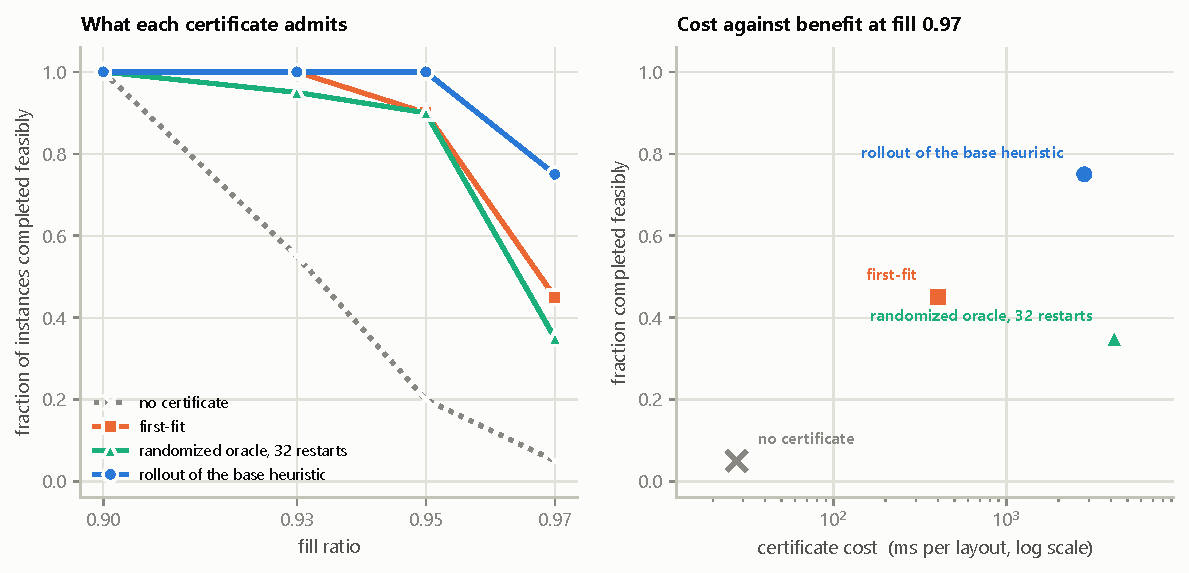
\includegraphics[width=\linewidth]{fig_certificate.pdf}
\caption{Left: what each certificate admits as the plate fills. Right: cost
against benefit at fill $0.97$. The randomized multistart certificate is the
highest admission sufficient test of the three and the worst filter, at ten
times the cost of first fit.}
\label{fig:certificate}
\end{figure}

Table~\ref{tab:certificates} shows $\cC_{\mathrm{rnd}}^{32}$ performing
\emph{worse} than $\cC_{\mathrm{ff}}$ despite certifying strictly more states,
and $\cC_{\mathrm{roll}}$ dominating both. Permissiveness itself is not the
mechanism: a sound certificate that accepts a superset removes no action the
narrower one allowed. What changes is which action the \emph{selector} then
takes. A wider accepted set exposes higher scoring candidates; the greedy
selector takes one; and the resulting state is completable exactly as
promised, but only along a trajectory this constructor never follows, because
$\cC_{\mathrm{rnd}}$'s witness is a random completion it will not reproduce.
$\cC_{\mathrm{roll}}$ directly tests whether the same constructor can complete
the current state. It is therefore the best filter in this experiment even
though it certifies fewer states. This result does not imply that a strict
certificate is always preferable. It indicates that the selector should be able
to follow the witness. The ordering may differ for a selector that searches
instead of committing greedily, which we have not tested.

\begin{rem}[The rule is relative, not absolute]
\label{rem:witness}
It follows that ``the best certificate'' is not a property of the certificate. We
confirmed the converse direction: for the learned policy, whose commit order is
its own, $\cC_{\mathrm{roll}}$, built on the \emph{base heuristic's}
continuation, gives $0.70$ feasibility at fill $0.97$ against
$\cC_{\mathrm{ff}}$'s $0.80$, at $17\times$ the cost. A certificate must be
matched to the constructor that consumes it, and we use $\cC_{\mathrm{roll}}$ for
the largest first constructor and $\cC_{\mathrm{ff}}$ for the policy accordingly.
\end{rem}

\subsection{Prediction cannot replace verification}
\label{sec:learned_cert}

$\cC_{\mathrm{roll}}$ costs a full $O(n^2WH)$ rollout for each query. We
therefore train a predictor of its result, which requires only one forward pass.
The predictor does not provide a reliable filter.

We collected $25\,258$ states from largest first rollouts on the train split at
fills $0.93$ to $0.97$, labeled each by whether the base heuristic completes from
it, and trained a network with two hidden layers on twelve features describing free
space and its usability (all computable in $O(nWH)$, an order below the rollout).
The split is by generated instance, stratified by fill: all states descended
from 96 instances form the training set ($19\,956$ states), and all states from
24 disjoint instances form validation ($5\,302$ states). This prevents sibling
states from the same trajectory leaking across the split. After $4\,000$ epochs,
validation AUC is $0.902$. At first fit's admission rate ($0.352$), the learned
predictor has recall $0.779$ and precision $0.764$, against first fit's $0.824$
and $0.809$, respectively.

Seven thresholds were fixed from validation
quantiles spanning admission rates from $0.010$ to $0.300$ and then evaluated on
20 disjoint test instances per fill. Feasibility at fill $0.95$ never exceeded
$0.20$, against
$0.90$ for $\cC_{\mathrm{ff}}$ and $1.00$ for $\cC_{\mathrm{roll}}$; at
several thresholds it was worse than no certificate at all.

This experiment does not prove that every learned model must fail; it exposes
a structural requirement that classification accuracy does not meet. A filter
is consulted $n$ times in sequence and one false admission can strand the
trajectory; a \emph{sound} test has no false admissions by construction, so
its only failure mode, admitting nothing, is detectable and recoverable. With
$E_t$ the event that step $t$ admits a state with no completion,
\begin{equation}
\Pr\Big(\bigcup_{t<n} E_t\Big)\;\le\;\sum_{t<n}\Pr(E_t),
\label{eq:union}
\end{equation}
which needs no independence assumption (errors along an autoregressive
trajectory are correlated: one wrong admission moves the state off the
training distribution). The bound makes the requirement quantitative: keeping
it below $0.1$ at $n=32$ requires the false admission probability at each step to be below
roughly $3\times10^{-3}$ on the states the decoder actually reaches, and it is
false positives that matter, because false negatives cost only coverage and
speed. Our predictor attains precision $1.0$ on validation only at an
admission rate of $0.010$, where almost nothing passes and the constructor
rejects every scored candidate at an average $992$ of a possible $1\,024$
filter calls per test instance at fill $0.95$. No threshold provides both useful
admission and reliable completion. Permissive settings strand facilities, while
strict settings admit almost no candidates. This result supports the use of a
learned surrogate to order candidates, but not to make the final decision for a
hard constraint. A learned witness generator followed by the same deterministic
verifier would remain sound.

\begin{rem}[Where this leaves learning]
\label{rem:soundness}
The distinction that matters for a hard guarantee is soundness, and a bare
classifier does not provide it. This is not an argument against learning in
constrained construction; it is an argument about where to put it. Feasibility
should be checked by a sound verifier, while learning can generate witnesses or
choose among verified options. Algorithm~\ref{alg:certified} uses the latter
arrangement.
\end{rem}

\fi

\subsection{Secondary certificate diagnostics}
The older full-regeneration decoder compared deterministic first fit, randomized
completion and a learned predictor. Randomized attempts accepted more prefixes,
but increased cost; the predictor reached validation AUC 0.902 and still admitted
states that its target rollout could not complete. These experiments distinguish
a rollout label from true completion feasibility and show why every accepted
completion must be verified. They do not establish the main quality-time claim.
Additional diagnostics and the certificate gallery are in the Online
Supplement; the complete run-level record includes the learned-selector failures
in the reproducibility archive.

\subsection{Completion-aware search with partial repair}
Algorithm~\ref{alg:certified} states M1, the principal method. Facilities are
visited in decreasing area in the first reconstruction and in randomized orders
afterwards. Positions are ranked by their exact marginal contribution. The
position already stored for the selected facility is appended to the top
$\kappa$ candidates, so a compatible commitment is always available. The search
continues until its post-initialization deadline.

\begin{algorithm}[H]
\caption{Completion-aware search with partial witness repair (M1).}
\label{alg:certified}
\footnotesize
\begin{algorithmic}[1]
\State $(ok,w)\gets\textsc{BestContact}(\emptyset)$; verify $w$
\State \textbf{if} $\lnot ok$ \textbf{then return} \textsc{Not Initialized}
\State $g_{\mathrm{best}}\gets w$; $J_{\mathrm{best}}\gets J(w)$
\State $B\gets\textsc{Clock}()+T$ \Comment{post-initialization deadline}
\While{$\textsc{Clock}()<B$}
  \State $P\gets\emptyset$ \Comment{committed prefix for one reconstruction}
  \For{facility $i$ in the selected order}
    \State $Q\gets$ top $\kappa$ legal positions by exact marginal score
    \State append $i$'s position in $w$ to $Q$ if absent
    \For{$p\in Q$ in decreasing score}
      \State $D\gets D(i,p;w)$
      \If{$D=\emptyset$}
        \State $w'\gets w\setminus\{i\}$ \Comment{reuse unchanged remainder}
      \ElsIf{$|D|\le4$}
        \State $w'\gets\textsc{Repair}(D\mid P,(i,p),w\setminus(D\cup\{i\}))$
      \Else
        \State $w'\gets\textsc{Failure}$
      \EndIf
      \If{$w'\ne\textsc{Failure}$}
        \State $g'\gets P\cup\{(i,p)\}\cup w'$
        \State $(ok,J',t_{\mathrm{done}})\gets\textsc{VerifyAndScore}(g')$
        \If{$t_{\mathrm{done}}>B$}
          \State discard $g'$; \textbf{return} $g_{\mathrm{best}}$
        \EndIf
        \If{$ok$}
          \State record $g'$ as an eligible completed layout
          \If{$J'>J_{\mathrm{best}}$}
            \State $g_{\mathrm{best}}\gets g'$; $J_{\mathrm{best}}\gets J'$
          \EndIf
        \State commit $(i,p)$ to $P$; $w\gets w'$; \textbf{break}
        \EndIf
      \EndIf
    \EndFor
    \If{the deadline is reached} \State \textbf{return} $g_{\mathrm{best}}$ \EndIf
  \EndFor
  \State $w\gets g_{\mathrm{best}}$ \Comment{start the next reconstruction from the incumbent}
\EndWhile
\State \textbf{return} $g_{\mathrm{best}}$
\end{algorithmic}
\end{algorithm}

The witness position in $Q$ has $D=\emptyset$, so the inner loop always has a
verified fallback unless the deadline interrupts it. In that case the separate
complete incumbent is returned. M0 replaces the repair branch by full
regeneration of all remaining facilities; like M1, it reuses the carried
witness action itself. R0 accepts only nonfallback proposals with $D=\emptyset$
and never calls repair, so it isolates witness reuse from repair. B3 evaluates the full completed
objective for each successful full regeneration and selects a non-worsening
continuation, which is fortified rollout. The learned selector studied later can
replace marginal ranking, but it is not used in the primary comparison.

With $r$ unplaced facilities, full first-fit completion costs $O(rWH)$ per
query. Partial generation costs $O(|D|WH)$ when $|D|\le4$, while the independent
whole-completion verifier remains $O(nWH)$. We therefore do not infer a speedup
from the complexity expression alone. We measure calls, repair sizes and
wall-clock quality. All matched-time experiments use $\kappa=32$.

\subsection{Comparison from the same initial layout}
\label{sec:sharedcomparison}

Table~\ref{tab:sharedmethods} lists the methods and controls used in the main
comparison. Every method starts
from the same verified best-contact layout $w_0$, keeps it as an incumbent, and
uses the same independent verifier. B1 isolates the value of intermediate
completion checks. B2 is a spatial large-neighborhood control: it removes 2 to
16 facilities near a random anchor and repacks them. B2S uses the identical
implementation but limits the destroy size to 2 to 4. B3 is fortified rollout.
M0, R0 and M1 have the same marginal candidate order. For every nonfallback
proposal, M0 regenerates all remaining facilities, R0 accepts only $D=0$, and
M1 applies Eq.~\eqref{eq:displaced} with a repair cap of four.
The guillotine and nonslicing instance families are described in
Section~\ref{sec:bench}.

\begin{table}[t]
\centering
\caption{Methods in the main comparison. All start from the same initial layout
and retain the best
verified complete layout found.}
\label{tab:sharedmethods}
\small
\begin{tabular}{@{}lp{0.24\linewidth}p{0.57\linewidth}@{}}
\toprule
ID & method & role \\
\midrule
B0 & initial witness & return $w_0$ without post-initialization search \\
B1 & final verification & randomized construction; verify only complete candidates \\
B2 & spatial destroy and repair & independent multi-facility improvement search \\
B2S & small spatial destroy and repair & B2 with destroy size restricted to 2 to 4 \\
B3 & fortified rollout & rank by completed objective and enforce non-worsening \\
M0 & full regeneration & marginal order; regenerate nonfallback proposals \\
R0 & reuse only & marginal order; accept nonfallback proposals only when $D=0$ \\
M1 & partial repair & marginal order with bounded witness reuse and repair \\
\bottomrule
\end{tabular}
\end{table}

\iflegacydetails

The parameters were selected on validation instances and then fixed:
$\kappa=32$, repair cap 4, and B2 destroy cap 16. The confirmation uses 50 new
instances in each $(\text{geometry},n)$ cell at fill 0.95. The guillotine family
is the original generator. The independent family starts from a five-rectangle
nonslicing pinwheel and permits local splits only while no full guillotine cut
exists. Rectangles are shrunk inside their source slots to the target fill. The
source packing is verified and withheld from every method. This family has a
different structural bias; we do not call it unbiased.

Each stochastic method has two evaluation seeds. We run each method once to
0.3 seconds and read its 0.1 second value from the same anytime trace.
Initialization generation and verification are measured once and charged to
every method. Its cell mean is 0.0030 to 0.0092 seconds, so the corresponding
nominal total budgets are 0.1030 to 0.1092 and 0.3030 to 0.3092 seconds. Quality
is compared only on the common initialized set. We first
average evaluation seeds within an instance, then use the instance as the
inference unit. Confidence intervals are percentile intervals from 5,000 paired
instance bootstrap samples. A difference of one percent of $J(w_0)$ was fixed as
the practical-effect threshold before this confirmation. The primary contrast
is pooled M1 minus B1 at 0.3 seconds on the 196 initialized instances. The four
cell intervals diagnose heterogeneity and are not treated as four additional
confirmatory tests.

Table~\ref{tab:sharedresult} reports improvement over the common initial layout,
and Figure~\ref{fig:sharedanytime} shows the pooled anytime and initialization views.
For the pooled primary contrast, M1 exceeds B1 by 4.64 percentage points (95\%
CI 3.67 to 5.60; win/tie/loss 151/1/44). The raw paired mean is 164.9 objective
units (95\% CI 110.7 to 220.9), and 150 of 196 instances meet the prespecified
one-percent practical threshold. Its cellwise point advantages range from 2.06
to 6.66 points. The result is not only incumbent
preservation: B1 and all other rows have the same safeguard. M1 also exceeds B3
and B2 in every cell. At $n=32$, M0 and M1 are statistically similar by 0.3
seconds. At $n=64$, M1 exceeds M0 by 3.57 percentage points on the guillotine
family (95\% CI 2.44 to 4.74) and 3.02 points on the nonslicing family (1.67 to
4.35). Partial repair therefore becomes useful relative to full regeneration at
the larger size.

\begin{table}[t]
\centering
\caption{Dense confirmation at fill 0.95 and a 0.3 second post-initialization
budget. Method columns are mean $100[J_m-J(w_0)]/J(w_0)$ on the common
initialized set. The last column is the paired percentage-point difference with
a pointwise 95\% bootstrap interval used to examine heterogeneity.}
\label{tab:sharedresult}
\small
\setlength{\tabcolsep}{3.6pt}
\begin{tabular}{@{}llrrrrrrrr@{}}
\toprule
geometry & $n$ & initialized & coverage & B1 & B2 & B3 & M0 & M1 & M1$-$B1 \\
\midrule
guillotine & 32 & 49/50 & 0.98 & 1.72 & 1.66 & 5.61 & 8.18 & \textbf{8.38} & 6.66 [5.09, 8.19] \\
guillotine & 64 & 50/50 & 1.00 & 4.44 & 0.96 & 2.60 & 4.32 & \textbf{7.89} & 3.45 [1.32, 5.54] \\
nonslicing & 32 & 47/50 & 0.94 & 1.79 & 1.82 & 5.49 & \textbf{8.54} & 8.34 & 6.55 [4.80, 8.26] \\
nonslicing & 64 & 50/50 & 1.00 & 4.10 & 0.92 & 2.51 & 3.14 & \textbf{6.16} & 2.06 [0.09, 4.03] \\
\bottomrule
\end{tabular}
\end{table}

\begin{figure}[t]
\centering

\includegraphics[width=\linewidth]{fig_completion_comparison.pdf}
\caption{Quality-time and initialization views for the dense confirmation.
Panel (a) pools the 196 initialized instances after averaging evaluation seeds;
bars are pointwise 95\% instance-bootstrap intervals. Each 0.1 second point is
read from the run that continues to 0.3 seconds. Panel (b) reports coverage and
Wilson intervals over all 50 attempted instances in each cell. G and N denote
guillotine and nonslicing geometry.}
\label{fig:sharedanytime}
\end{figure}

The mechanism logs support a limited explanation. The mean displaced-set size
is 2.12 and 2.24 at $n=32$, and 3.57 and 4.23 at $n=64$, for the guillotine and
nonslicing families respectively. Only 2.5\% to 6.8\% of attempted nonempty
repairs succeed, but unchanged witness reuse is common and M1 records 32.2 to
43.1 verified nonfallback completions per run. M0 records 10.6 to 31.3. No final
verification failure occurs. These data show that repair is selective, not that
it decides completion feasibility.

The 0.1 second sensitivity gives the same M1 over B1 direction in all four
cells, with paired advantages from 1.58 to 5.39 percentage points. The boundary
study at fill 0.90 is different. At $n=32$, M1 and B1 are statistically similar
by 0.3 seconds. At $n=64$, B1 has the higher point estimate in both geometry
families; the nonslicing paired difference is $-2.50$ points (95\% CI $-4.22$
to $-0.72$). Completion handling is therefore useful when density and a short
budget make complete unfiltered constructions rare. It is overhead outside that
regime.

\subsection{Earlier certificate and selector diagnostics}
\label{sec:legacydiagnostics}

The following experiments use the earlier full-regeneration decoder and learned
selectors. They are retained to document initialization coverage, certificate
compatibility and learning failure modes. They are not part of the matched-time
claim in Section~\ref{sec:sharedcomparison}.

\begin{table}[t]
\centering
\caption{Full sweep with the legacy full-regeneration certified decoder, $20$ instances per cell. Coverage is the
fraction for which a verified witness is found at $s_0$. It is identical for the
two policy seeds because initial witness generation does not use the selector.
All 1,320 returned layouts across the two seeds were independently verified as
feasible. Effort is the number of completion attempts at the empty plate,
randomized after the first; per step certificate calls use a single attempt.}
\label{tab:coverage}
\small
\begin{tabular}{@{}llrrrr@{}}
\toprule
& & \multicolumn{4}{c}{coverage at witness effort} \\
\cmidrule(lr){3-6}
$n$ & fill ratio & 1 & 8 & 32 & 128 \\
\midrule
32 & $0.75$ & 1.00 & 1.00 & 1.00 & 1.00 \\
32 & $0.80$ & 1.00 & 1.00 & 1.00 & 1.00 \\
32 & $0.85$ & 0.95 & 1.00 & 1.00 & 1.00 \\
32 & $0.90$ & 0.65 & 0.70 & 0.80 & \textbf{0.95} \\
32 & $0.95$ & 0.05 & 0.05 & 0.05 & 0.05 \\
\midrule
64 & $0.75$ & 1.00 & 1.00 & 1.00 & 1.00 \\
64 & $0.80$ & 0.95 & 1.00 & 1.00 & 1.00 \\
64 & $0.85$ & 1.00 & 1.00 & 1.00 & 1.00 \\
64 & $0.90$ & 1.00 & 1.00 & 1.00 & 1.00 \\
64 & $0.95$ & 0.45 & 0.45 & 0.45 & 0.45 \\
\bottomrule
\end{tabular}
\end{table}

Table~\ref{tab:coverage} shows the coverage associated with the guarantee.
Coverage is high when the plate is loose and decreases when it is tight. A total
of $128$ randomized completions
lift $n=32$, fill $0.90$ from $0.65$ to $0.95$ at $0.08$\,s per instance and
do nothing in either cell at fill $0.95$. These are coverage rates, not
feasibility rates; every returned layout in every cell is verified feasible,
while the guided heuristic answers every instance with empirical success and
no guarantee. Which decoder a practitioner wants depends on whether an
unverified layout has any value.

\iflegacydetails
\paragraph{Coverage depends on the generator}
The coverage column of Table~\ref{tab:coverage} is a property of the initial
witness generator alone, so the generator is the component to improve.
The deterministic baseline is already bottom left fill in decreasing area, the
standard packing rule. Table~\ref{tab:witfrontier} compares several
alternatives on the six cells whose baseline coverage remains below one at
effort $128$. Three further cells dip below one only at effort $1$ ($n=32$
fill $0.85$ and $n=64$ fill $0.80$ at $0.95$, dense $n=64$ fill $0.90$ at
$0.99$): restarts already close them in Table~\ref{tab:coverage}, every
generator below except width order also holds $0.95$ to $1.00$ there, and the
archive's result file reports all nine cells. Three findings emerge on the six
open cells. The sort key matters more than randomization:
height order beats
$128$ randomized restarts of the area order in every one of them. A
best contact rule processes rectangles in decreasing area and puts each at the
legal position maximizing total shared edge length with already placed
rectangles and the plate walls, breaking ties in row major bottom left order. It reaches coverage
$0.95$ to $1.00$ everywhere at under $10$\,ms per instance, where the baseline
reaches $0.05$ to $0.78$. And a time limited complete solver adds little
beyond it: CP-SAT decision packing certifies $0.95$ to $1.00$ within $10$\,s
per instance, and in the hardest cell ($n=64$, fill $0.95$) the $9$\,ms
heuristic covers more instances than the complete solver's ten second budget.

\begin{table}[t]
\centering
\caption{Coverage of alternative initial witness generators from the empty plate on the
six cells whose baseline coverage remains below one at witness effort $128$.
All witnesses pass the same
deterministic verifier. Heuristic generators run in at most $10$\,ms per
instance; CP-SAT rows give coverage within the stated wall clock limit (mean
solve time $0.06$ to $2.4$\,s on solved instances). The $1$\,s row is read off
per instance solve times on one otherwise idle machine and is
timing sensitive by an instance or two; the $10$\,s row is stable across
repeated runs.}
\label{tab:witfrontier}
\footnotesize
\setlength{\tabcolsep}{2.5pt}
\begin{tabular}{@{}lrrrrrr@{}}
\toprule
 & \multicolumn{3}{c}{full sweep ($20$/cell)} & \multicolumn{3}{c}{dense ($100$/cell)} \\
\cmidrule(lr){2-4}\cmidrule(lr){5-7}
generator & 32/$0.90$ & 32/$0.95$ & 64/$0.95$ & 32/$0.90$ & 32/$0.95$ & 64/$0.95$ \\
\midrule
bottom left fill, area order (baseline) & 0.65 & 0.05 & 0.45 & 0.78 & 0.09 & 0.28 \\
\quad $+128$ randomized restarts        & 0.95 & 0.05 & 0.45 & 0.90 & 0.09 & 0.28 \\
bottom left fill, height order          & 1.00 & 0.40 & 0.75 & 0.95 & 0.31 & 0.69 \\
bottom left fill, perimeter order       & 0.85 & 0.20 & 0.25 & 0.84 & 0.15 & 0.41 \\
bottom left fill, width order           & 0.05 & 0.00 & 0.00 & 0.09 & 0.00 & 0.00 \\
best contact, area order                & 1.00 & 0.95 & 1.00 & 0.98 & 0.96 & 1.00 \\
CP-SAT decision packing, $1$\,s         & 1.00 & 0.90 & 0.30 & 1.00 & 0.96 & 0.24 \\
CP-SAT decision packing, $10$\,s        & 1.00 & 1.00 & 0.95 & 1.00 & 1.00 & 0.95 \\
\bottomrule
\end{tabular}
\end{table}

Theorem~\ref{thm:certified} does not depend on the generator. Consequently, the
legacy decoder inherits whichever coverage rate the generator supplies. Run end to end with the
best contact witness and the exact marginal selector introduced below, the
decoder answers $19/20$ and $20/20$ of the full sweep instances at fill $0.95$ and
$n=32$ and $n=64$, and $98/100$, $96/100$ and $100/100$ of the dense cells at
$(n,\text{fill})=(32,0.90)$, $(32,0.95)$ and $(64,0.95)$,
with every one of the $333$ returns verified feasible and the carried witness
supplying at most
$6.8\%$ of commitments. The low dense coverage in Table~\ref{tab:coverage}
therefore reflects the baseline generator, not the feasible-continuation invariant.

\paragraph{Comparison with the initial witness}
The legacy full-regeneration decoder verifies a complete witness $w_0$ before its
first commitment, so it could return $w_0$ unchanged. Feasibility of its
returns is therefore guaranteed by construction. We next measure how much the
certified deviations from $w_0$ improve the objective.
Table~\ref{tab:witnessgap} answers it with the paired comparison the carried
witness makes possible: the returned layout against the witness it started
from, per instance.

\begin{table}[t]
\centering
\caption{Certified returns against their own initial witness, full sweep at
witness effort $128$, both policy seeds pooled. $J(w_0)$ is the objective of
the verified first fit witness the decoder could have returned unchanged;
$\Delta$ is the paired mean improvement of the returned layout over it, and
won/lost counts instance and policy seed returns (each covered instance
appears once per seed, so $40$ pairs are $20$ instances). The witness is
identical for
the two seeds because $w_0$ precedes selection.}
\label{tab:witnessgap}
\small
\begin{tabular}{@{}rrrrrrr@{}}
\toprule
$n$ & fill & pairs & $J(w_0)$ & returned & $\Delta$ & won/lost \\
\midrule
32 & $0.75$ & 40 & 2\,294.7 & 2\,667.6 & $+372.9$ ($+16.2\%$) & 40/0 \\
32 & $0.80$ & 40 & 1\,871.4 & 2\,231.7 & $+360.3$ ($+19.3\%$) & 40/0 \\
32 & $0.85$ & 40 & 2\,079.4 & 2\,421.3 & $+342.0$ ($+16.4\%$) & 40/0 \\
32 & $0.90$ & 38 & 1\,958.4 & 2\,214.7 & $+256.3$ ($+13.1\%$) & 38/0 \\
32 & $0.95$ &  2 & 2\,101.7 & 2\,432.9 & $+331.1$ ($+15.8\%$) &  2/0 \\
\midrule
64 & $0.75$ & 40 & 7\,182.7 & 8\,451.4 & $+1\,268.7$ ($+17.7\%$) & 40/0 \\
64 & $0.80$ & 40 & 6\,751.0 & 7\,804.8 & $+1\,053.7$ ($+15.6\%$) & 40/0 \\
64 & $0.85$ & 40 & 6\,590.1 & 7\,602.7 & $+1\,012.6$ ($+15.4\%$) & 40/0 \\
64 & $0.90$ & 40 & 6\,757.4 & 7\,672.9 & $+915.5$ ($+13.5\%$) & 40/0 \\
64 & $0.95$ & 18 & 6\,851.8 & 7\,514.4 & $+662.6$ ($+9.7\%$) & 18/0 \\
\bottomrule
\end{tabular}
\end{table}

Across the earlier certified policy runs, all efforts and both seeds, the
certified deviations improve on the witness in $2{,}189$ of the $2{,}202$
returns and worsen it in $13$. (These counts are specific to the
selected by the policy population; the certified runs of the two later experiments,
$771$ exact marginal and $333$ best contact returns, were separately verified
feasible.) The stored witness is used mainly as a fallback. It supplies no
commitments at fills up to $0.90$ and at most
$2.6\%$ of commitments in the hardest cell ($n=64$, fill $0.95$). The pattern
repeats on the disjoint dense cells reported later in
Table~\ref{tab:denseconfirm}, with pooled improvements of $15.1$ and $9.3$
percent at $n=32$, fills $0.90$ and $0.95$, and $13.1$ and $7.2$ percent at
$n=64$. All $13$ worsened returns lie in those dense cells, the largest
regression being $298$ objective units: nothing in the mechanism forces the
returned layout to dominate $w_0$, because the decoder commits certified
deviations in selector order and never revisits them. The regeneration script
(\code{witness\_gap.py}) reproduces $w_0$ exactly and checks that its success
pattern matches the recorded coverage flags on all $96$ certified return
populations.

\paragraph{Effect of learning inside the mechanism}
We next evaluate whether the learned selector improves the objective inside the
certified mechanism. We run the identical decoder (same witnesses, same
seed, same $\kappa$, same carried witness fallback) with the exact marginal
largest first rule as the selector; coverage is unchanged by construction, and
the script asserts that the certified flags match the policy runs cell for
cell ($771$ returns across the sweep and dense cells, every one verified
feasible). Table~\ref{tab:certgreedy} reports the paired differences on the full
sweep at effort $128$. At $n=64$ the selector without training is ahead in every
cell and against both seeds, by $103$ to $288$ objective units ($1$ to $4\%$
of $J$); the dense cells repeat this ($+71$ to $+195$). At $n=32$ the
differences stay within $\pm52$ units and change sign across cells and seeds
on the full sweep (the single instance cell at fill $0.95$ changes to $-166$
against seed 2), while on the dense cells the policy is consistently but
modestly ahead ($6$ to $41$ units). The greedy selector pays with certificate
work where the plate is tight: at $n=64$, fill $0.95$ it is rejected $2\,236$
times and takes $4.9\%$ of its commitments from the carried witness, against
at most $2.6\%$ for the policy. These results show that learned ranking is an
optional selector inside the certified mechanism. At $n=64$, it is not the best
available selector.

\begin{table}[t]
\centering
\caption{The legacy certified decoder with a selector that requires no training, full sweep at
witness effort $128$. $\Delta$ is greedy minus policy on the identical
certified return population, positive when the exact marginal rule is ahead of
that seed's policy.}
\label{tab:certgreedy}
\small
\begin{tabular}{@{}rrrrrr@{}}
\toprule
$n$ & fill & pairs & $J$ greedy & $\Delta$ seed 1 & $\Delta$ seed 2 \\
\midrule
32 & $0.75$ & 20 & 2\,719.1 & $+51.7$ & $+51.3$ \\
32 & $0.80$ & 20 & 2\,230.8 & $+7.6$ & $-9.4$ \\
32 & $0.85$ & 20 & 2\,432.0 & $+11.5$ & $+9.9$ \\
32 & $0.90$ & 19 & 2\,221.6 & $+16.4$ & $-2.5$ \\
32 & $0.95$ &  1 & 2\,346.3 & $-7.5$ & $-165.7$ \\
\midrule
64 & $0.75$ & 20 & 8\,640.1 & $+169.6$ & $+207.9$ \\
64 & $0.80$ & 20 & 8\,039.0 & $+180.8$ & $+287.7$ \\
64 & $0.85$ & 20 & 7\,722.6 & $+103.0$ & $+137.0$ \\
64 & $0.90$ & 20 & 7\,809.8 & $+124.1$ & $+149.6$ \\
64 & $0.95$ &  9 & 7\,687.6 & $+171.9$ & $+174.5$ \\
\bottomrule
\end{tabular}
\end{table}

\fi

\fi

Coverage is an initializer property here, not a methodwise output metric. The
legacy comparison further showed that the carried witness prevents output
infeasibility but does not by itself improve its objective, and that an exact
marginal selector can match or exceed the learned selector. We therefore use a
common best-contact initializer and training-free selectors in the primary
comparison. Selected witness-frontier and selector diagnostics are reported in
the Online Supplement, with complete tables in the reproducibility archive.

%%%%%%%%%%%%%%%%%%%%%%%%%%%%%%%%%%%%%%%%%%%%%%%%%%%%%%%%%%%%%%%%%%%%%%%%%%%%%%
\section{Experimental design}
\label{sec:protocol}

\subsection{A generated benchmark}
\label{sec:bench}
Repeating a solver on a fixed brief measures solver variability, not instance
variability, so the two reference scenarios cannot support a statement about how
a method behaves across problems. We generate a held out suite and treat the
\emph{instance} as the unit of analysis.

\paragraph{Feasibility by construction}
Sampling facility sizes independently produces instances that cannot be packed
at high density, and a suite containing impossible instances measures nothing.
The original suite is built from a guillotine partition, recursively slicing
the plate into $n$ disjoint integer rectangles and shrinking each inside its own
slot.

The second family starts from a tiled five-rectangle pinwheel with no full
horizontal or vertical guillotine cut. A source rectangle is selected and split
at an integer coordinate. The split is accepted only if the resulting tiling
still has no full guillotine cut. This procedure is repeated until the tiling has
$n$ source slots. The rectangles are then reduced by a common scale factor,
rounded down to integer dimensions, and enlarged one cell at a time without
leaving their respective slots until the target fill is reached. The nonslicing
condition is checked on the complete source tiling before this reduction. After
the reduction, gaps are present and the same full-cut test for a tiling is no
longer applicable. We therefore do not claim that the reduced layout is
nonslicing under a definition that allows dead space.

For both families, the lower-left corners of the source slots give a feasible
witness. Its boundary and overlap conditions are independently verified before
any solver is run, but the coordinates are withheld from every method. The
implementation is in \code{rl\_layout/v2/bench.py}, the structural checks are in
\code{rl\_layout/v2/test\_bench\_families.py}, and the experimental entry point is
\code{rl\_layout/v2/run\_completion\_comparison.py} in the accompanying archive.

\paragraph{Design}
The suite crosses four facility counts, $n\in\{8,16,32,64\}$, with three fill
ratios, $f\in\{0.40,0.60,0.75\}$, at $20$ instances per cell: $240$ instances.
Five extensions follow the same construction from disjoint seeds.
Section~\ref{sec:results_density} adds $f\in\{0.80,0.85,0.90,0.95\}$ at $n=32$
($80$) and $f\in\{0.85,0.90,0.95\}$ at $n=64$ ($60$);
Section~\ref{sec:results_scale} adds $n\in\{96,128,192,256\}$ at $f=0.85$ and
$f=0.95$, with plates enlarged in proportion so facilities do not shrink to the
minimum size ($180$). The certified sweep adds the missing $n=64,f=0.80$ cell
($20$). Finally, the frozen decoders are run on a confirmatory family of $100$
new instances in each $n\in\{32,64\}$ by $f\in\{0.90,0.95\}$ cell ($400$), and
a small plate family at $n=8$ ($60$), sized so that constraint programming can
prove optima, supports the gap study of Section~\ref{sec:results_bench}.
These legacy diagnostic suites contain $1\,040$ distinct held out instances.
The main comparison adds 200 dense confirmation instances and 80
boundary-study instances under separate tags. Every source packing is verified.
Achieved fill ratios match their targets to within $0.001$. Plate aspect ratio, the type
inventory, the preference matrix, boundary preferences and the objective
constants are redrawn per instance; facility sizes come from the partition and
types are drawn independently of geometry.

\paragraph{Splits}
Train, validation and test draw from disjoint generator seed ranges, so an
instance evaluated at test time cannot have been optimized in training. Instance
identity is $(\text{family},\text{split},n,f,\text{index})$ and is reproducible
from the seed. The earlier policy confirmation is tagged
\texttt{dense100\_v3}. The new comparison families use separate v4 tags;
they are disjoint from training, validation and all earlier test cells.

\subsection{Primary comparison protocol}
The dense study crosses two geometry families and $n\in\{32,64\}$ at fill
0.95, with 50 attempted instances per cell. The boundary check uses the same
four cells at fill 0.90, with 20 attempts per cell. The common best-contact
initializer succeeds on 196 of 200 dense instances and 79 of 80 boundary
instances. Quality comparisons use these fixed common initialized sets.

All methods are run once to a 1.0 second post-initialization cutoff. Values at
0.1 and 0.3 seconds are read from the same anytime trace. The dense study uses
two evaluation seeds per stochastic method and the boundary study uses three.
Evaluation seeds are averaged within an instance before any paired comparison.
The instance is the inference unit, and intervals use 5,000 paired instance
bootstrap samples. A difference of one percent of $J(w_0)$ is the fixed
practical-effect threshold.

The tuned parameters are $\kappa=32$, M1 repair cap 4, and B2 destroy cap 16.
B2 draws the destroy size uniformly from 2 through the cap, selects the nearest
facility centers to a random anchor, optionally shuffles their decreasing-area
order, and samples from a restricted list of the four strongest among 12
candidate positions. Only a complete independently verified improvement can
replace the incumbent. On 20 disjoint validation instances at $n=64$, fill
0.95, and 0.3 seconds, B2 caps 4, 8, 12 and 16 improved the initial objective
by 1.06\%, 1.00\%, 1.15\% and 1.34\%, respectively; cap 16 was then fixed.
B2S repeats the test implementation with cap 4 to test small destroy sizes
directly.

\subsection{Methods}
The primary methods B0 to B3, B2S, M0, R0 and M1 are defined in
Table~\ref{tab:sharedmethods}. They are classical CPU implementations and share
the initial layout, objective, time limit and verifier. The following methods
belong to the earlier diagnostic experiments.

\begin{itemize}
\item \textbf{Classical search}: shelf packing; lattice constrained simulated
annealing at $8\,192$ and $45\,000$ proposals; tabu search
\citep{Glover1989Tabu} over single facility moves; and a lattice genetic
algorithm with uniform crossover and elitism. Annealing and tabu use periodic
greedy polish and a common budget of $45\,000$ objective calls.
Constraining annealing to the lattice is itself worth $4.4\%$ on
\textsc{office} and raises \textsc{clinic} feasibility from $20\%$ to $100\%$;
we report against this stronger version. Tabu's tenure and start and the GA's
population and memetic setting are chosen on validation like every other
hyperparameter: tabu keeps the constructive start (steepest single facility
moves cannot repair a random dense start), and the memetic variant was
rejected for exceeding the evaluation budget tenfold without improving on its
compliant counterpart.
\item \textbf{Masked constructive methods without training}: greedy with largest first
order; greedy with joint choice of facility and position; regret $k$ insertion for
$k\in\{2,4,8\}$; beam search over insertion decisions at widths $1$ to $64$; and
beam search with the order fixed to largest first.
\item \textbf{Methods without training and with certificate guidance}: largest first and joint greedy
with the certificate filter of Section~\ref{sec:certified} and an argmax fallback.
These are empirical heuristics, not instances of Theorem~\ref{thm:certified}.
\item \textbf{Learned}: a constructive policy trained with PPO
\citep{Schulman2017PPO}; its heuristic variant with certificate guidance; and its
legacy full-regeneration variant with a carried witness. This last method uses
the invariant of Theorem~\ref{thm:certified}, but not the partial repair of
Algorithm~\ref{alg:certified}. Architecture and hyperparameters are in
\ref{app:policy}.
\end{itemize}

Beam width and regret $k$ are selected on the \emph{validation} split for the
objective comparison of Section~\ref{sec:results_bench}, and the test split is
evaluated once with them fixed. The density cells of
Section~\ref{sec:results_density} report the whole sweep instead, because the
finding there is the pattern of collapse across widths. On the two reference
scenarios, single instances with no validation counterpart, the best setting
is taken on the scenario itself; that favors the baselines without training, and
we flag it there rather than reporting a $p$ value.

\subsection{Which policy covers which instances}
\label{sec:coverage_map}
The encoder concatenates pair features of length $n$, so one checkpoint serves one
facility count (Section~\ref{sec:limitations}). No single policy spans the suite,
and Table~\ref{tab:datamap} states exactly which instances a learned method was
run on and which are comparisons of methods without training. Aggregate instance counts
elsewhere in the paper refer to held out \emph{test} instances; training and
validation instances are drawn from disjoint seed ranges and are never evaluated.

\begin{table}[t]
\centering
\caption{Datasets, and the policies evaluated on them. Training budgets and
wall clock differ by policy family and are listed per checkpoint in
Table~\ref{tab:training} of \ref{app:policy}; training cost is per policy, not
amortized across rows.}
\label{tab:datamap}
\footnotesize
\setlength{\tabcolsep}{3pt}
\begin{tabular}{@{}llrll@{}}
\toprule
dataset & $n$ & inst. & policies & trained on \\
\midrule
generated, main    & 8, 16   & 120 & none               & not used \\
                   & 32      &  60 & 3 seeds, env order & train, $f{\le}0.75$ \\
                   & 64      &  60 & see density rows   & not used \\
generated, density & 32      &  80 & 2 seeds, own order & train, $f{=}0.75$ to $0.90$ \\
                   & 64      &  60 & 2 seeds, own order & train, $f{=}0.75$ to $0.90$ \\
generated, certified only & 64 & 20 & 2 seeds, own order & frozen; $f{=}0.80$ \\
generated, dense confirm & 32, 64 & 400 & 2 seeds, own order & frozen checkpoints \\
same initial layout, dense & 32, 64 & 200 & none & not used \\
same initial layout, boundary & 32, 64 & 80 & none & not used \\
generated, large   & 96 to 256 & 180 & none (fixed $n$)   & not used \\
generated, exact   & 8       &  60 & none               & not used \\
reference scenarios & 32     &   2 & 1 per scenario     & that scenario \\
MCNC / GSRC        & 33 to 300 &   5 & none (other obj.)  & not used \\
QAPLIB             & 12 to 30  &  32 & none (other obj.)  & not used \\
\bottomrule
\end{tabular}
\end{table}

\subsection{Cost accounting}
\label{sec:cost}
One ``evaluation'' does not mean the same work for every method, so we separate
four units: full objective evaluations, $O(n^2)$ each; candidate position scores,
one exact marginal for one facility at one position; network forward passes,
one of which scores all $O(WH)$ positions; and wall clock, with hardware
named. Learned inference uses a GPU and classical solvers vectorized CPU code;
the comparisons our conclusions rest on are between constructive methods
scoring the same position grid, and the missing CPU only inference figure is
flagged in Section~\ref{sec:limitations}. The primary comparison
does not mix CPU and GPU methods. It records wall time from one continuous
anytime run, including scoring, repair and verification. A candidate is admitted
only if its independent verification and objective evaluation both finish by
the cutoff. Work already in flight may finish later, but that candidate is
discarded; the largest function-return overrun was 9.8 ms and the latest admitted
event was at 0.999998 s. Measured initialization time is reported separately and
charged equally to every method. The v5
comparison used one AMD Ryzen 7 9700X CPU process on Windows 10, with Python
3.7.16 and NumPy 1.21.5; the exact metadata are stored with the result file.
The CP-SAT audit used OR-Tools 9.15 in the separate exact environment.

\subsection{Statistics}
For the main comparison, quality is defined on the fixed common
initialized set. Stochastic evaluation seeds are averaged within each instance,
then paired differences are bootstrapped over instances. We report raw and
initial-objective-normalized differences, win/tie/loss counts, and the
fixed one-percent practical threshold. Every shorter budget is a prefix
of the longest run. The primary dense contrast is M1 minus B1 at 1.0 seconds;
contrasts with R0, B2S and M0 test reuse, repair scale and regeneration,
respectively.

For the earlier diagnostic experiments, the following protocol is retained.
Every method is attempted on every instance in the cells assigned to it.
Objective comparisons are paired only on instances for which both methods return
feasible layouts. We normalize by the best \emph{feasible} objective achieved on
that instance, because raw values differ by an order of magnitude between cells
with $8$ and $64$ facilities. We report the mean paired gap, a $95\%$
bootstrap confidence interval over instances, a Wilcoxon signed rank test on
paired differences with Holm correction across the family, and the number of
instances on which each method wins. For binary reliability we report exact
binomial confidence intervals. In the prespecified dense confirmation, guided and
unfiltered decoders are paired instance by instance using the exact two sided
McNemar test, with Holm correction across all twelve selector and cell comparisons.
Coverage and feasibility conditional on return are analyzed separately for the
selective decoder.

%%%%%%%%%%%%%%%%%%%%%%%%%%%%%%%%%%%%%%%%%%%%%%%%%%%%%%%%%%%%%%%%%%%%%%%%%%%%%%
\section{Results}
\label{sec:results}

\subsection{Dense results from the same initial layout}
\label{sec:sharedresult}
At the 1.0 second cutoff, M1 exceeds B1 by 5.93 percentage points on the
196 initialized dense instances (95\% paired bootstrap interval 4.99 to 6.88;
win/tie/loss 156/0/40). The raw paired mean is 224.5 objective units (172.2 to
276.5), and 152 instances meet the fixed one-percent practical threshold.
The cellwise M1 minus B1 differences are 7.79, 4.33, 7.86 and 3.88 points in
Table~\ref{tab:sharedresult} order; all four intervals exclude zero.

Comparisons with the direct controls give the following results. Pooled M1 minus R0 is 6.39 points
(5.89 to 6.92; 195/0/1), so reuse without nonempty repair does not explain the
gain. M1 minus B2 is 7.02 points (6.54 to 7.52; 196/0/0), and M1 minus B2S is
6.33 points (5.84 to 6.82; 195/0/1). Restricting B2 to the same small destroy
scale therefore does not close the gap.

The comparison with full regeneration depends on the cutoff. The pooled M1
minus M0 differences are 1.18 points at 0.1 seconds (0.58 to 1.75), 1.05 points
at 0.3 seconds (0.46 to 1.67), and 0.25 points at 1.0 second ($-0.42$ to 0.92).
At 0.1 seconds, the pooled difference is mainly due to the two $n=32$ cells;
the M1 point estimate is lower than M0 by 0.31 and 0.33 points in the two $n=64$
cells. Thus, the early difference is not uniform across sizes. At one second,
the interval establishes neither a difference nor equivalence between partial
repair and full regeneration. The early results are consistent with the intended
role of partial repair, since it repacks only the displaced rectangles. They do
not support a general claim about longer runs or deployment settings.

\begin{table}[t]
\centering
\caption{Dense study at fill 0.95 and a 1.0 second post-initialization cutoff.
Method columns are mean $100[J_m-J(w_0)]/J(w_0)$ on the common initialized
set. The last column is the paired M1 minus B1 difference with a pointwise
95\% bootstrap interval.}
\label{tab:sharedresult}
\footnotesize
\setlength{\tabcolsep}{2.1pt}
\begin{tabular}{@{}llrrrrrrrrrr@{}}
\toprule
geometry & $n$ & init. & cov. & B1 & B2 & B2S & B3 & M0 & R0 & M1 & M1$-$B1 \\
\midrule
guillotine & 32 & 49/50 & .98 & 1.72 & 2.40 & 3.51 & \textbf{9.63} & 9.04 & 2.43 & 9.51 & 7.79 [6.04,9.44] \\
guillotine & 64 & 50/50 & 1.00 & 4.44 & 1.41 & 1.62 & 3.69 & 8.00 & 2.31 & \textbf{8.76} & 4.33 [2.25,6.37] \\
nonslicing & 32 & 47/50 & .94 & 1.79 & 2.64 & 3.71 & 9.53 & \textbf{10.15} & 2.86 & 9.65 & 7.86 [6.18,9.53] \\
nonslicing & 64 & 50/50 & 1.00 & 4.10 & 1.38 & 1.78 & 3.60 & 7.78 & 2.70 & \textbf{7.98} & 3.88 [2.00,5.81] \\
\bottomrule
\end{tabular}
\end{table}

\begin{figure}[t]
\centering

\includegraphics[width=\linewidth]{fig_completion_comparison.pdf}
\caption{Quality time and initialization views for the dense study. Panel (a)
pools the 196 initialized instances after averaging evaluation seeds; bars are
pointwise 95\% instance-bootstrap intervals. The 0.1 and 0.3 second points are
prefixes of runs that continue to 1.0 second. Panel (b) reports coverage and
Wilson intervals over 50 attempted instances per cell. G and N denote
guillotine and nonslicing geometry.}
\label{fig:sharedanytime}
\end{figure}

\subsection{Mechanism and timing checks}
The mean proposed displaced-set size ranges from 1.95 to 2.72 across the dense
cells. Only 2.19\% to 3.91\% of attempted nonempty repairs of size at most four
succeed. Still, the successful repair branch produces 6,215 incumbent updates
and 92\% of M1's logged objective gain, compared with 1,380 updates from
unchanged reuse. These are descriptive event counts, not independent samples.
They agree with the paired R0 contrast: the nonempty repair branch, rather than
reuse alone, carries the improvement.

B2's mean destroy size is 8.88 to 9.06, while B2S's is 2.99 in every cell.
Thus the B2S comparison directly checks the concern that B2 loses only because
its neighborhoods are larger. M1 processes 55.0 to 80.8 verified nonfallback
completions per run, and M0 processes 35.7 to 59.6. No intermediate or final
verification failure occurs.

The independent result auditor regenerates every instance, verifies all 8,820
stored budget layouts, recomputes their objectives, and checks every budget row
against its eligible trace prefix. The largest objective and trace errors are
both zero. In-flight work produces 194 candidates that finish after the cutoff;
all are discarded. No admitted event is later than 0.999998 seconds, although a
nonpreemptive call can return up to 9.8 ms after the cutoff.

\subsection{Boundary at fill 0.90}
The boundary check is based on 80 attempted instances, of which 79 share a
verified initial layout. At 1.0 second, pooled M1 minus B1 is 0.23 points
($-0.75$ to 1.22); this interval does not establish a difference. M1 minus M0
is $-1.87$ points ($-2.60$ to $-1.17$). In the four cells, M1 improves the
initial objective by 14.60\%, 13.44\%, 13.84\% and 13.07\%, while M0 gives
16.17\%, 15.48\%, 14.90\% and 15.85\%. Partial repair is therefore useful
relative to the direct reuse and spatial controls at fill 0.95, but it is not a
general replacement for full regeneration when the plate is less tight.

\iflegacydetails
\subsection{Calibration on the reference scenarios}
\label{sec:results_scenarios}
Table~\ref{tab:main} reports \textsc{office}. The masked constructive action set
is worth more than any correction inside the improvement formulation: a greedy
rule with no learned parameters reaches $3\,380.2$ using $528$ objective
evaluations, above the reference annealer's $3\,269.9$ at $59\,987$. Training free
nonmyopic search inside the same action set reaches $3\,497.2$, and the trained
policy $3\,529.3$ at $32$ evaluations. On \textsc{clinic} the corresponding
figures are $4\,116.5$, $4\,124.7$ and $4\,163.1$.

\begin{table}[t]
\centering
\caption{\textsc{office}, 64 layouts, identical objective. Candidate scores are
exact marginals, not objective evaluations (Section~\ref{sec:cost}).}
\label{tab:main}
\small
\setlength{\tabcolsep}{4pt}
\begin{tabular}{@{}lrrrr@{}}
\toprule
method & $J$ & feas.\ \% & obj.\ evals & ms \\
\midrule
shelf packing (no search)                & 2\,931.6 & 100 & 1 & $\approx$0 \\
tabu search, random start                & 2\,662.7 & 0   & 44\,929 & 1\,360 \\
tabu search, greedy start                & 3\,361.8 & 100 & 44\,929 & 7\,207 \\
memetic GA                               & 3\,177.0 & 100 & 144\,318 & 8\,871 \\
SA 45\,000 $+$ polish \emph{(reference impl.)} & 3\,269.9 & 100 & 59\,987 & 1\,950 \\
SA 45\,000, lattice                      & 3\,414.8 & 100 & 61\,267 & 1\,520 \\
\midrule
masked greedy, area order                & 3\,359.5 & 100 & 32 & 7 \\
masked greedy, joint                     & 3\,380.2 & 100 & 528 & 88 \\
masked beam search, width 32             & 3\,435.0 & 100 & 32 & 8\,136 \\
\textbf{masked regret 4 insertion}       & \textbf{3\,497.2} & 100 & 1 & 864 \\
\midrule
\textbf{constructive policy (learned)}   & \textbf{3\,529.3} & \textbf{100} & \textbf{32} & \textbf{18} \\
\bottomrule
\end{tabular}
\end{table}

The action space supplies most of the gain over classical search. Nonmyopic
selection without training supplies most of the remainder. Learning adds only $0.9\%$
over the best procedure in the same action set on both scenarios.

\subsection{The benchmark at moderate density}
\label{sec:results_bench}
The picture changes when the same methods are run on instances none of them was
trained on. Beam width and regret $k$ were selected on the \emph{validation}
split ($60$ instances at $n=32$, fills $0.40$ to $0.75$, disjoint seeds), which
chose width $32$ and $k=4$; the test split was then evaluated once with those
settings fixed. All comparisons below are paired on the instances both methods
solved feasibly. Pairing removes the composition confound that arises when
reliability differs, but the jointly solved population is itself an outcome of
the methods compared, so reliability is always reported alongside conditional
quality rather than folded into it.

Beam search without training has the best result. Against beam search of width 32,
the three suite trained policies lose by $75.3$, $89.7$ and $101.7$ objective
points ($p\le4.9\times10^{-8}$, $n=57$ paired instances), and so does every
alternative without training: regret $4$ by $88.1$, largest first greedy by $108.8$,
lattice annealing by $42.0$, tabu search from the constructive start by $105.4$
($p=3.3\times10^{-9}$), and the genetic algorithm by $448.7$ on the $33$ of $60$
instances it solves at all. Paired against the greedy layout it starts from,
tabu gains $3.5$ points ($95\%$ CI $[2.2,5.1]$, $p=5\times10^{-11}$),
statistically significant and practically negligible at $0.1\%$ of the
objective: at this budget the single facility polish does not escape the
start's basin. The policies improve only reliability, and only slightly:
$60/60$ against beam search's $57/60$
(exact binomial intervals $[0.94,1.00]$ against $[0.86,0.99]$).

At moderate density feasibility is nearly free and beam search optimizes the
objective better than a single policy pass. Section~\ref{sec:results_density}
shows where increasing density reverses the operational priority.

\fi

\subsection{Secondary calibration and the small-instance audit}
\label{sec:results_bench}
On the two hand-authored scenarios, masked constructive search supplies most of
the improvement over translation-based search, but learning adds only 0.9\%
over the best training-free procedure in the same action set. On 60 held-out
moderate-density instances, beam search without training has the best paired
objective and solves 57, compared with 60 for the policies. These results keep
learning out of the primary contribution; supporting tables and complete
run-level tests are reported in the Online Supplement and archive, respectively.

\paragraph{Small-instance objective audit}
Paired differences say which method is better, not whether any of them is good.
To measure that we freeze a dedicated small plate family from the same
generator ($n=8$, fills $0.40$ to $0.75$, $20$ instances each, mean facility
area $6$ to $10$ so plates stay at $66$ to $195$ cells). The CP-SAT model
\citep{GoogleCPSAT} has
integer lower-left coordinates $X_i\in[0,W-w_i]$ and
$Y_i\in[0,H-h_i]$, interval variables of fixed size, and a native
\textsc{NoOverlap2D} constraint. For every nonzero pair, an allowed-assignment
table has columns $(u,v,q)$, where $u=X_j-X_i$, $v=Y_j-Y_i$, and
$q=\operatorname{round}(10^4 w_{\mathrm{adj}}c_{ij})$. Boundary coefficients are rounded at the
same scale and attached to reified wall-contact variables. The no-overlap bonus
is constant on $\cF$ and is added without rounding.

Let $a_\ell(g)$ denote an unrounded active pair or wall term, let $M$ be the
number of such terms and let $s=10^4$.
For every feasible layout,
\begin{equation}
 \widehat J(g)=\beta_{\max}+\frac{1}{s}
 \sum_{\ell=1}^{M}\operatorname{round}(s a_\ell(g)),
 \qquad |J(g)-\widehat J(g)|\le\delta:=\frac{M}{2s}.
\label{eq:quantbound}
\end{equation}
Thus a CP-SAT upper bound $\widehat U$ transfers to the real objective as
$U=\widehat U+\delta$, and an optimizer of $\widehat J$ is within $2\delta$ of
the real optimum. CP-SAT proves 45 of 60 \emph{quantized} models optimal within
600 seconds and returns bounds for the other 15. The audit independently checks
all returned layouts and reevaluates their real objective. The largest
$\delta$ is $0.00215$ and the largest observed $|J-\widehat J|$ is $0.000322$.
We therefore make no claim of literal exact optimality for the real-valued
objective.

\begin{table}[t]
\centering
\caption{Small-instance calibration at $n=8$. The first three numeric columns
are real-objective shortfalls from the returned CP-SAT solution on the 45
quantized models proved optimal. The last column uses the transferred real upper
bound $U$ on all 60 instances. Objectives and bounds are positive here, so
$(U-J)/U$ upper-bounds the relative gap to the unknown real optimum. Regret 4 is
infeasible on one instance and is excluded rather than imputed.}
\label{tab:gaps}
\small
\setlength{\tabcolsep}{4pt}
\begin{tabular}{@{}lrrrr@{}}
\toprule
method & mean & median & max & certified upper bound \\
\midrule
beam width 32          & \textbf{0.40\%} & \textbf{0.19\%} & 2.66\% & $\le$0.85\% \\
SA 45\,000, lattice    & 1.48\% & 0.85\% & 9.79\% & $\le$1.74\% \\
regret 4 insertion     & 1.94\% & 1.41\% & 6.05\% & $\le$2.35\% \\
tabu 45\,000, greedy start & 2.62\% & 1.96\% & 7.31\% & $\le$2.88\% \\
largest first greedy   & 2.77\% & 2.13\% & 7.31\% & $\le$3.00\% \\
\bottomrule
\end{tabular}
\end{table}

The ranking replicates the paired comparison on this small family. The result is
only a calibration at $n=8$ for the same objective. It does not bound an unknown
gap at $n=32$ or $64$, and it does not transfer to QAPLIB.

\iflegacydetails
\subsection{The density regime}
\label{sec:results_density}
Table~\ref{tab:density} and Figure~\ref{fig:density} report the $100$ held out
instances at $n=32$ and fills $0.75$ to $0.95$.

\begin{table}[t]
\centering
\caption{Density sweep, $n=32$, $20$ held out instances per cell. Each entry is
raw mean emitted objective / feasibility rate. The raw mean includes infeasible
outputs and is shown only for traceability; all quality inference uses jointly
feasible instances. All constructive methods use the identical
masked action set. Rows labeled ``guided'' add the certificate of
Section~\ref{sec:certified} with an uncertified argmax fallback. Policies were
trained at fills $0.75$ to $0.90$, so the
$0.95$ column is extrapolation for them. Rows marked $\times K$ use $K$ times
the decoding budget and are operating points, not matched budget comparisons.
Policy rows show the second trained seed; Figure~\ref{fig:density} pools both
seeds, which is why its $\times16$ point at fill $0.95$ is $0.75$ (seed 1:
$0.70$) against this table's $0.80$.}
\label{tab:density}
\footnotesize
\setlength{\tabcolsep}{1.5pt}
\begin{tabular}{@{}lccccc@{}}
\toprule
method & $f{=}0.75$ & $0.80$ & $0.85$ & $0.90$ & $0.95$ \\
\midrule
SA 45\,000, lattice              & 2719/1.00 & 2287/0.95 & 2304/0.85 & 2001/0.20 & 1944/0.00 \\
tabu 45\,000, greedy start       & 2724/1.00 & 2236/1.00 & 2435/1.00 & 2205/1.00 & 2169/0.25 \\
GA 45\,000, lattice              & 1936/0.00 & 1563/0.00 & 1491/0.00 & 1405/0.00 & 1330/0.00 \\
free order beam, width 16        & 2732/0.95 & 2261/0.85 & 2266/0.55 & 1966/0.20 & 1744/0.00 \\
joint greedy                     & 2676/0.75 & 2173/0.60 & 2231/0.35 & 1990/0.20 & 1843/0.00 \\
largest first greedy             & 2720/1.00 & 2234/1.00 & 2433/1.00 & 2203/1.00 & 2133/0.20 \\
largest first $+$ beam 16        & 2731/1.00 & 2253/1.00 & 2462/1.00 & 2209/1.00 & 1323/0.20 \\
\midrule
joint greedy, guided             & 2741/0.95 & 2298/0.95 & 2476/0.90 & 2149/0.70 & 1840/0.10 \\
largest first, guided            & 2720/1.00 & 2234/1.00 & 2432/1.00 & 2209/1.00 & 2387/0.90 \\
\midrule
policy, uncertified, $\times16$  & 2752/1.00 & 2317/1.00 & 2511/1.00 & 2298/1.00 & 2458/0.80 \\
\textbf{policy, guided}           & 2673/1.00 & 2239/1.00 & 2434/1.00 & 2246/1.00 & 2359/0.95 \\
\quad $\times8$                  & \textbf{2743/1.00} & \textbf{2318/1.00} & \textbf{2506/1.00} & \textbf{2310/1.00} & \textbf{2506/1.00} \\
\bottomrule
\end{tabular}
\end{table}

\begin{figure}[t]
\centering

\includegraphics[width=\linewidth]{fig_density.pdf}
\caption{Left: the fraction of instances on which a method produces any
overlap free layout. Right: solution quality among what survives, as a paired gap
to the best value for each instance. The policy curve pools both trained seeds;
Table~\ref{tab:density} lists seed 2.}
\label{fig:density}
\end{figure}

\paragraph{One step masking is not enough}
Every method that relies on one step legality alone loses feasibility as the
plate fills, and they do so in an informative order. Procedures that choose
\emph{which} facility to commit by immediate objective gain fail earliest (the
joint greedy rule is at $0.35$ by fill $0.85$), while largest first, the weakest
selector we implement, survives to $0.90$. Feasibility at density is governed by
the commit order, not by the sophistication of the position choice. Annealing,
which is not constructive at all, collapses earliest of the methods that are
fully feasible at fill $0.75$ (to $0.20$ by fill $0.90$), and the lattice
genetic algorithm never reaches feasibility at any of these fills. Tabu search,
seeded with the largest first layout, holds feasibility exactly as far as its
seed does ($1.00$ through fill $0.90$; $0.25$ against the seed's $0.20$ at
$0.95$) and moves the objective by a few points: at $45\,000$ evaluations
against the constructor's $32$, the improvement neighborhood preserves what
construction achieved and adds little.

\paragraph{Certificate guidance}
Filtering the leading largest first candidates with $\cC$ lifts empirical
feasibility at fill $0.95$ from $0.20$ to $0.90$ and the objective from $2\,133$
to $2\,387$, for $159$\,ms per layout and no training. This row uses the guided
heuristic and its argmax fallback, so it is an empirical result rather than a
consequence of Theorem~\ref{thm:certified}. It also shows that filtering does not
substitute for a sensible order: joint greedy reaches only $0.10$, because its
top $\kappa$ candidates are often rejected and the heuristic then falls back.

\paragraph{The difference is reliability, and mostly not objective value}
As in Section~\ref{sec:results_bench}, quality is compared only on jointly
feasible instances; reliability is reported separately
(Table~\ref{tab:reliability}), since raw means charge failures an arbitrary
penalty and per method feasible means reward unreliability.

The guided reliability gain is large. At fill $0.95$ the guided policy solves
$20/20$ instances; its exact 95\% interval is $[0.83,1.00]$. Largest first and
its beam of width 16 solves $4/20$, regret $8$ solves $3/20$, and annealing and
free order beam solve none.

On objective value, restricted to instances both methods solved, the picture is
much narrower than the raw means suggest. The policy is significantly better than
largest first greedy at fill $0.85$ ($-73.4$, $p=1.7\times10^{-3}$) and at fill
$0.90$ ($-107.1$, $p=3.8\times10^{-6}$), and better than largest first with a beam
at $0.90$ ($-100.9$, $p=4.8\times10^{-5}$). It is \emph{not} distinguishable from
regret $k$ insertion at any density, and at fills $0.75$ and $0.95$ no comparison
reaches significance at all. The $2\,506$ against $2\,387$ at fill $0.95$ in
Table~\ref{tab:density} is a difference between populations, not between methods,
and we do not claim it.

In short, \emph{regret $k$ insertion
matches the learned policy's solution quality wherever it can produce a layout,
and produces one far less often}: $11$ of $20$ at fill $0.90$ against $20$, and
$3$ of $20$ at fill $0.95$ against $20$.

\begin{table}[t]
\centering
\caption{Reliability at fill $0.95$, $n=32$, $20$ instances, with exact binomial
intervals. A rate of $1.00$ on twenty instances supports a lower bound of
$0.83$, not certainty. Policy rows are seed 2; seed 1 gives $20/20$ for the
guided $\times8$ decoder and $14/20$ unfiltered $\times16$.}
\label{tab:reliability}
\small
\begin{tabular}{@{}lrcr@{}}
\toprule
method & feasible & rate & 95\,\% CI \\
\midrule
policy, guided heuristic $\times8$  & 20/20 & 1.00 & $[0.83,1.00]$ \\
policy, unfiltered $\times16$       & 16/20 & 0.80 & $[0.56,0.94]$ \\
tabu 45\,000, greedy start          &  5/20 & 0.25 & $[0.09,0.49]$ \\
largest first greedy                &  4/20 & 0.20 & $[0.06,0.44]$ \\
largest first $+$ beam 16           &  4/20 & 0.20 & $[0.06,0.44]$ \\
regret 8 insertion                  &  3/20 & 0.15 & $[0.03,0.38]$ \\
SA 45\,000, lattice                 &  0/20 & 0.00 & $[0.00,0.17]$ \\
free order beam 16                  &  0/20 & 0.00 & $[0.00,0.17]$ \\
GA 45\,000, lattice                 &  0/20 & 0.00 & $[0.00,0.17]$ \\
\bottomrule
\end{tabular}
\end{table}

\paragraph{Disjoint confirmation with 100 instances}
The preceding rates use $20$ instances per cell. Before inspecting any new
outcome, we froze both policy checkpoints, both decoders and their budgets, then
generated the disjoint \texttt{dense100\_v3} family. Table~\ref{tab:denseconfirm}
reports all four prespecified cells. Heuristic rows are empirical feasibility
among the $100$ emitted candidates; selective rows are coverage. Thus a value in
one kind of row must not be read as the other.

\begin{table}[t]
\centering
\caption{Dense confirmation, $100$ new instances per cell. Heuristic entries are
empirical feasibility; selective entries are coverage, with feasibility among
returns equal to 1.00 throughout. Policy entries show seed 1/seed 2. Certified
coverage is invariant to the seed because witness generation precedes selection.}
\label{tab:denseconfirm}
\footnotesize
\setlength{\tabcolsep}{2.5pt}
\begin{tabular}{@{}lcccc@{}}
\toprule
& \multicolumn{2}{c}{$n=32$} & \multicolumn{2}{c}{$n=64$} \\
\cmidrule(lr){2-3}\cmidrule(lr){4-5}
method & $f{=}0.90$ & $f{=}0.95$ & $f{=}0.90$ & $f{=}0.95$ \\
\midrule
largest first, unfiltered       & 0.92 & 0.25 & 1.00 & 0.42 \\
largest first, guided           & 1.00 & 0.81 & 1.00 & 0.85 \\
policy, unfiltered              & 0.97/0.98 & 0.40/0.40 & 0.69/0.73 & 0.02/0.02 \\
policy, guided                  & 1.00/1.00 & 0.97/0.91 & 1.00/0.99 & 0.70/0.86 \\
\midrule
legacy certified decoder, effort 1 (cov.)   & 0.78 & 0.09 & 0.99 & 0.28 \\
legacy certified decoder, effort 128 (cov.) & 0.90 & 0.09 & 1.00 & 0.28 \\
\bottomrule
\end{tabular}
\end{table}

At fill $0.95$, guidance raises largest first from $25/100$ to $81/100$ at
$n=32$ and from $42/100$ to $85/100$ at $n=64$. The two policies move from
$40/100$ to $97/100$ and $91/100$ at $n=32$, and from $2/100$ to $70/100$ and
$86/100$ at $n=64$. In paired exact McNemar tests, all six improvements remain
significant after Holm correction ($p_{\mathrm{Holm}}\le7.2\times10^{-15}$ at
$n=32$ and $p_{\mathrm{Holm}}\le1.2\times10^{-10}$ at $n=64$). At fill $0.90$
the ceiling leaves less room: largest first improves $92/100$ to $100/100$
($p_{\mathrm{Holm}}=0.031$), while the two $n=64$ policies improve by 31 and 26
instances with no losses ($p_{\mathrm{Holm}}\le1.5\times10^{-7}$).

At $n=32$, coverage with effort 128 is $0.90$ (95\% CI $[0.824,0.951]$) at
fill $0.90$ and $0.09$ ($[0.042,0.164]$) at fill $0.95$. At $n=64$ it is
$1.00$ ($[0.964,1.000]$) and $0.28$ ($[0.195,0.379]$), respectively. All $882$ layouts
returned across these confirmatory certified runs were independently verified
feasible, bringing the certified policy count to $2,202$ returns with zero
violations. Conditional objective comparisons do not overturn the distinction:
on jointly solved cases at fill $0.90$, the decoder with effort 128 differs from the
guided decoder by $0.0/0.0$ objective units at $n=32$ and $-0.4/0.0$ at $n=64$
(seed 1/seed 2, certified minus guided on the maximized objective, so the one
nonzero entry is a deficit of $0.4$ units for the certified decoder). At fill $0.95$
the paired sets are small and
the signs differ across seeds, so we make no population wide quality claim.

\paragraph{Cost}
A policy decode with certificate guidance costs $32$ objective evaluations and $51$
to $269$\,ms (eight samples $0.5$ to $1.8$\,s); the guided constructor without
training costs $0.4$ to $1.0$\,s; full budget annealing costs $1.6$ to $2.9$\,s with a
lower objective value. Certificate evaluations, rather than the network, dominate at the
highest density (up to $2\,368$ rejections per batch of $20$). The selective
decoder with effort 128 takes $74$ to $93$\,ms per $n=32$ instance and $227$ to
$321$\,ms at $n=64$ on the confirmation family, including abstentions and
verification; its cost is not directly comparable to a heuristic that always
completes, so coverage stays beside timing rather than folded into it.

\subsection{Scale}
\label{sec:results_scale}

The density experiments above fix $n=32$. Stranding is a coordination failure
among facilities, so the facility count is the other axis on which one step
legality should become a looser relaxation of viability. We test it two ways:
with a policy at $n=64$, the largest count at which we could train one, and with
constructors without training on a separate suite of $96$ to $256$ facilities, whose
plates are enlarged in proportion so that facilities do not shrink to the
minimum size.

\paragraph{Policy guidance at $n=64$}
Table~\ref{tab:n64} reports the original cells with 20 instances. At fill $0.90$,
largest first and regret $8$ retain $1.00$ and $0.95$ feasibility while annealing,
free order beam and joint greedy fall to $0.05$, $0.05$ and $0.00$. The two plain
policies reach $0.05$ and $0.45$, and first fit guidance raises both to $1.00$. At
fill $0.95$, policies guided by first fit reach $0.35/0.70$ against a best
rate of $0.15$ among methods without training. Raw objectives include infeasible outputs and are
shown only for traceability, not quality inference.

\begin{table}[t]
\centering
\caption{$n=64$, $20$ held out instances per cell, raw mean emitted objective /
empirical feasibility. Raw means include infeasible outputs and support no
quality inference. Policy rows show seed 2; seed 1 is reported in the text and the
seed spread is not used for an inferential claim. Guided rows allow an
uncertified fallback.}
\label{tab:n64}
\footnotesize
\setlength{\tabcolsep}{2pt}
\begin{tabular}{@{}lcccc@{}}
\toprule
method & $f{=}0.75$ & $0.85$ & $0.90$ & $0.95$ \\
\midrule
SA 45\,000, lattice        & 8691/0.95 & 7695/0.45 & 7173/0.05 & 7222/0.00 \\
tabu 45\,000, greedy start & 8660/1.00 & 7729/1.00 & 7798/1.00 & 7331/0.15 \\
GA 45\,000, lattice        & 6078/0.00 & 5746/0.00 & 4637/0.00 & 5325/0.00 \\
free order beam, width 4   & 9041/1.00 & 7896/0.50 & 7399/0.05 & 6868/0.00 \\
joint greedy               & 8975/0.95 & 7866/0.40 & 7534/0.00 & 7164/0.00 \\
largest first greedy       & 8647/1.00 & 7724/1.00 & 7794/1.00 & \textbf{7315}/0.15 \\
regret 8 insertion         & 9015/1.00 & 8072/1.00 & 7967/0.95 & 7330/0.05 \\
\midrule
policy, uncertified        & not run & 7395/0.90 & 7378/0.45 & 6742/0.00 \\
\textbf{policy, guided} ($\cC_{\mathrm{ff}}$, seed 2)
                           & not run & \textbf{7527}/\textbf{0.95} & \textbf{7629}/\textbf{1.00} & 7119/\textbf{0.70} \\
\quad with $\cC_{\mathrm{roll}}$ & not run & not run & 7485/0.90 & 6896/0.50 \\
\bottomrule
\end{tabular}
\end{table}

\paragraph{The certificate choice holds across scales}
The ordering of Remark~\ref{rem:witness} persists at $n=64$: first fit
guidance gives $0.35/0.70$ feasibility at fill $0.95$ against $0.15/0.50$ for
rollout, at about $1/26$ of the cost. The disjoint confirmation agrees
($0.70/0.86$ guided by first fit, $0.02/0.02$ unguided, $0.85$ guided
largest first) while retaining a policy seed spread of 16 percentage points; its fill $0.90$
unfiltered rates ($0.69/0.73$) also show that the original cells' $0.05$ and
$0.45$ were imprecise estimates from 20 instances, the guided rates ($1.00/0.99$)
being unchanged.

\paragraph{Larger instances}
The ladder of methods without training runs on $96$ to $256$ facilities ($15$ instances per
cell at fill $0.85$, $30$ at $0.95$; the full table is in the Online
Supplement, S8). At fill $0.85$ every setting is feasible; at fill $0.95$,
witness compatibility separates them. Rollout raises feasibility from
$0.57/0.53$ to $0.90/0.90$ at $n=96/128$, whereas first fit changes the four
size specific rates from $0.57,0.53,0.70,0.83$ to $0.53,0.57,0.63,0.83$. Thus,
the mismatched witness does not improve feasibility. Rollout is omitted above $n=128$ because each
query costs $O(n^2WH)$ and may be invoked $\kappa$ times per commitment; that
is recorded rather than hidden.

\subsection{QAPLIB: when feasibility is trivial, improvement wins}
\label{sec:results_qap}

The generated suite does not provide standard instances that have been studied
for decades or distances to a \emph{proven} optimum. The quadratic assignment
problem \citep{Koopmans1957QAP} provides both. It is also closely related to our problem:
at fill ratio $1.0$, with $n$ unit square facilities on $n$ grid locations and a
pure flow times distance objective, lattice placement \emph{is} a QAP. General
QAPLIB instances need not arise this way (their distance matrices are not always
grid metrics), so we treat them as an analogous control with proven optima
rather than as instances of Eq.~\eqref{eq:objective}.
The pairwise objective admits the same exact marginal decomposition as
Eq.~\eqref{eq:objective} and HPWL (assigning facility $i$ to location $\ell$
adds $\sum_{j\ \text{placed}} A_{ij}B_{\ell,\pi(j)}+A_{ji}B_{\pi(j),\ell}$, a
third objective for Proposition~\ref{prop:marginal}'s pattern), so the
constructive machinery transfers verbatim. Feasibility, however, is trivial:
any injective assignment completes and the certificate passes vacuously. A
swap neighborhood also exists at every state, because no empty space is needed
to use it. This is the regime most favorable to classical improvement
search.

We run the suite of methods without training on $32$ QAPLIB instances \citep{Burkard1997QAPLIB}
with proven optimal values (families \textsc{nug}, \textsc{had}, \textsc{scr},
\textsc{rou}, \textsc{chr}, \textsc{els}, \textsc{tai}a; $n=12$ to $30$; the
largest, \textsc{nug30}, was closed by \citealp{Anstreicher2002Nug30}). Swap
simulated annealing and tabu search in Taillard's robust configuration
\citep{Taillard1991Robust}, with per assignment tabu, random tenure in
$[n/2,3n/2]$ and aspiration on the incumbent, parameters taken from the
literature and not tuned, receive the paper's standard budget of $45\,000$
full evaluation equivalents, with swap deltas charged at $8n$ terms and tabu iterations at the
$2n^2$ delta update rate. Constructive insertion (busiest first greedy, the
analogue of largest first; regret $4$; beam $32$) consumes what its candidate
counts imply: $7$, $67$ and $209$ evaluation equivalents respectively. No
learned method appears because each checkpoint is specific to one facility count
and objective (Section~\ref{sec:coverage_map}).

\begin{table}[t]
\centering
\caption{QAPLIB: mean gap to the proven optimum by instance family, and overall.
All methods share the objective implementation validated by the marginal
telescoping test; permutations are verified before scoring. Budgets in
full evaluation equivalents; wall clock on the same CPU as
Table~\ref{tab:density}.}
\label{tab:qap}
\footnotesize
\setlength{\tabcolsep}{3.4pt}
\begin{tabular}{@{}lrrrrrr@{}}
\toprule
 & & \multicolumn{3}{c}{constructive insertion} & \multicolumn{2}{c}{swap search} \\
\cmidrule(lr){3-5}\cmidrule(lr){6-7}
family & inst. & greedy & regret 4 & beam 32 & SA & tabu \\
\midrule
\textsc{nug} 12 to 30 & 15 & 19.5\% & 12.5\% & 8.9\% & 0.63\% & \textbf{0.20\%} \\
\textsc{had} 12 to 20 &  5 &  6.2\% &  5.5\% & 2.2\% & \textbf{0.04\%} & 0.22\% \\
\textsc{scr} 12 to 20 &  3 & 36.4\% & 20.8\% & 15.7\% & 0.22\% & \textbf{0.00\%} \\
\textsc{rou} 12 to 20 &  3 & 14.0\% & 12.0\% & 8.0\% & 2.08\% & \textbf{0.00\%} \\
\textsc{chr} 12 to 20 &  3 & 119.9\% & 103.7\% & 30.3\% & 7.74\% & \textbf{0.49\%} \\
\textsc{els19}      &  1 & 315.0\% & 193.6\% & 241.6\% & \textbf{4.21\%} & 17.74\% \\
\textsc{tai}a 20 to 25 & 2 & 18.2\% &  8.8\% & 8.7\% & 2.11\% & \textbf{0.15\%} \\
\midrule
mean gap            & 32 & 37.1\% & 26.1\% & 17.7\% & 1.51\% & \textbf{0.74\%} \\
median gap          & 32 & 18.5\% & 12.2\% & 9.2\% & 0.70\% & \textbf{0.00\%} \\
proven optimum found & 32 & 0 & 0 & 1 & 9 & \textbf{24} \\
evaluations/instance &   & 7 & 67 & 209 & 45\,000 & 45\,000 \\
\bottomrule
\end{tabular}
\end{table}

Table~\ref{tab:qap} gives a clear result. Swap tabu
search finds the proven optimum on $24$ of $32$ instances and has a mean gap
of $0.74\%$. Annealing has a mean gap of $1.51\%$, while the best constructive method reaches
a median gap of $9.2\%$. Two points should be noted. First, the constructive methods
spend $200$ to $6\,000$ times fewer
evaluations, and beam's $9.2\%$ at $209$ evaluation equivalents is a statement
about value per evaluation, not competitiveness at the budget. Second, the
\textsc{chr} and \textsc{els} families, whose flow matrices have a few dominant
entries, are known to defeat myopic insertion, and they do: greedy insertion
exceeds $100\%$ gap exactly where the literature predicts.

When the plate is dense and facilities have different shapes,
the swap and displacement neighborhoods contain few useful feasible moves.
Annealing and free order beam solve $0$ of $20$ instances at fill $0.95$
(Table~\ref{tab:reliability}), while construction with certified completion can
still return solutions. In QAPLIB, feasibility is trivial and every swap is
feasible. Improvement search then obtains solutions within a small fraction of
the proven optima, and the constructive methods are not competitive at the same
budget. Thus, the two experiments differ in whether the improvement neighborhood
remains useful. The QAPLIB optima evaluate the methods without training on that
separate objective. They do not bound the unknown gaps of the fixed-shape layout
problem.

\subsection{Standard floorplanning: representation fails before certification matters}
\label{sec:results_mcnc}

Every instance used so far is either manually defined or produced by our own
generator, and a generator that guarantees a feasible packing could plausibly
also be producing instances that are unrepresentatively easy to pack. We
therefore tested the method on the field's standard instances (MCNC
\textsc{ami33} and \textsc{ami49}, GSRC \textsc{n100}, \textsc{n200},
\textsc{n300}) with the objective the floorplanning literature actually uses,
half perimeter wirelength, in the fixed outline formulation, allowing the
$90^\circ$ block rotations that literature allows
\citep{Murata1996SequencePair,Adya2003FixedOutline}.

\paragraph{Instances and conversion}
Blocks, nets and terminals come from the standard MCNC/GSRC files under the
usual center pin simplification. Coordinates are divided by an integer chosen
for each instance ($6$ for \textsc{ami33}, $33$ for \textsc{ami49}, $3$ for GSRC)
because our legality masks are dense over the plate, and the outline is fixed
by area from a dead space target at aspect ratio $1$, with $90^\circ$
rotations allowed. Under this conversion HPWL is comparable across our own
methods but \emph{not} against published floorplanning numbers, which use full
resolution and a different pin model. Integer flooring also changes shapes and
packing possibilities, so achieved dead space after conversion is not identified
with a published full-resolution result. The conversion is stated in full in the
Online Supplement (S7).

\paragraph{Transfer of the method}
The constructive apparatus is independent of the objective.
Placing a block can only grow the bounding boxes of the nets it belongs to, and
that growth depends on the already placed pins of those nets and never on the
unplaced ones, so HPWL admits an exact marginal exactly as
Eq.~\eqref{eq:objective} does, now at cost $O(\text{nets containing } i)$
rather than $O(|\cP_t|)$. We verified this to floating point precision on all
five benchmarks: marginals accumulated along a construction reproduce the total
wirelength of the layout they build to a relative error below $5\times10^{-15}$,
for arbitrary commit orders.

\paragraph{Results on standard benchmarks}
Our constructive methods place all blocks of all five benchmarks at $15\%$ dead
space, a common fixed outline setting, and fail below it: the tightest outline any
of them fills is $15\%$ dead space on four benchmarks and $6\%$ on
\textsc{ami49}. Published topological fixed outline methods report substantially
tighter outlines on these benchmark families
\citep{Murata1996SequencePair,Chang2000BStar,Adya2003FixedOutline}.
We are not competitive on these instances and do not claim to be.

The reason is representational. Topological representations such as sequence
pairs and B*-trees \citep{Murata1996SequencePair,Chang2000BStar}
enumerate only compact packings, so area tightness is a property of the
encoding. Absolute lattice placement, which is what makes the feasibility mask
and the certificate possible at all, must instead \emph{find} compactness by
search. Restricting candidate positions to the classical corner point set (the
plate edges and the right and top edges of placed blocks) raised achieved
utilization at extreme density from $0.68$ to $0.85$ and made the constructor
$60\times$ faster, and still does not close the gap.

\paragraph{Implication for the certificate}
These benchmarks cannot directly evaluate the certificate claim. The certificate matters in the
regime where a constructor is operating near the density at which the instance is
still packable \emph{by that constructor}; on MCNC and GSRC our constructors run
out of room at $15\%$ dead space, far from the regime, and there the three
certificate settings produce identical wirelength on every benchmark. The one
exception is consistent with this: on \textsc{ami49} the first fit
certificate reaches $6\%$ dead space where no certificate reaches $10\%$, but
its wirelength is $55\%$ higher.

The phenomenon this
paper characterizes requires an instance family that is packable at high density
by the method under study, and it requires knowing that it is, which is exactly
what the generated suite of Section~\ref{sec:bench} provides through its witness
and what no standard benchmark provides. The generated suite is therefore
needed for this evaluation. However, the result is limited to this operating
regime.

\fi

\subsection{Secondary boundary studies}
\label{sec:results_density}
\label{sec:results_scale}
\label{sec:results_qap}
\label{sec:results_mcnc}
Four older studies delimit the claim. First, unfiltered one-step construction
loses completion reliability as fill approaches 0.95; this motivated explicit
completion handling. Second, feasibility experiments up to 256 facilities test
packing rules rather than the proposed M1 search and are not evidence of learned
or certified scalability. Third, QAPLIB removes geometric feasibility and favors
swap improvement, but its optima say nothing about the gap of the layout
objective. Fourth, direct transfer to integer-converted MCNC/GSRC floorplans is
not competitive with topological fixed-outline methods; conversion changes
rectangle geometry and dead space. Selected tables are in the Online Supplement
and the complete negative record is in the archive. None of these studies is
used to strengthen the main comparison.

%%%%%%%%%%%%%%%%%%%%%%%%%%%%%%%%%%%%%%%%%%%%%%%%%%%%%%%%%%%%%%%%%%%%%%%%%%%%%%
\section{Discussion}
\label{sec:discussion}

The comparison from the same initial layout clarifies the interpretation of the
paper. A stored feasible continuation is not by itself evidence of better
performance. Final
verification with an incumbent has the same feasible-return coverage and the
same non-worsening output property. What matters is whether intermediate
completion work changes the quality-time tradeoff.

The results depend on density and cutoff. At fill 0.95, partial repair is better than
final-verification construction, both spatial destroy controls and reuse without
repair. The reuse contrast and event decomposition show that successful
nonempty repairs matter. However, the one-second comparison with full witness
regeneration does not establish a difference. At fill 0.90, complete
constructions are easier and full regeneration is better. Maintaining and
repairing a witness is useful near a packing barrier; outside that regime its
extra structure need not improve the incumbent.

This interpretation also separates two incumbents that were mixed in the older
formulation. The compatible completion is state dependent and supports the next
commitment. The best complete layout is global to the run and protects output
quality. Fortified rollout couples these roles through a completed-objective
acceptance rule. M1 permits marginal ranking, but keeps the roles separate and
verifies every full candidate before it can update the output incumbent.

The earlier penalty, mask and learning experiments remain diagnostic. A reward
penalty does not enforce feasibility, and a one-step mask can strand facilities.
A predictive filter with AUC 0.902 does not replace verification. Beam and regret
controls also show that learning is not a general replacement for search. These
results motivate completion-aware construction, but the primary computational
claim rests on the classical matched-time experiment.

The small CP-SAT and QAPLIB studies have limited roles. The former calibrates
methods for the same objective at $n=8$, with an explicit integer-to-real error
allowance. The latter shows that swap search is strong when geometric
feasibility is absent. Neither study supplies an optimality bound for the dense
32- or 64-facility cells.

%%%%%%%%%%%%%%%%%%%%%%%%%%%%%%%%%%%%%%%%%%%%%%%%%%%%%%%%%%%%%%%%%%%%%%%%%%%%%%
\section{Limitations}
\label{sec:limitations}

\begin{enumerate}
\item \textbf{The primary evidence is short-horizon.} The dense confirmation
uses 50 instances per cell, two evaluation seeds and post-initialization cutoffs
of 0.1, 0.3 and 1.0 seconds. It supports a short-budget claim, not long-run
dominance. The boundary check has only 20 attempted instances per cell.

\item \textbf{Initialization remains incomplete.} Best-contact coverage is 0.94
to 1.00 in the new dense cells. Quality inference is therefore conditional on
the common initialized set. No result establishes that the initializer covers
all feasible instances.

\item \textbf{Repair controls are not exhaustive.} B2 is a documented,
validation-tuned spatial destroy-and-repair search, and B2S checks destroy sizes
2 to 4. They are not a full adaptive large-neighborhood search portfolio.
Different destroy rules, CP-SAT repair, or longer tuning may improve the
control. M1's cap of four and exact marginal candidate order are also empirical
choices.

\item \textbf{The representation and objective limit external validity.}
The core experiments use fixed-orientation axis-aligned rectangles on a lattice,
without corridors or doors. Rotation is enabled only in the separate MCNC/GSRC
transfer study. Integer conversion changes those benchmark geometries, and the
absolute-coordinate representation is less competitive than topological fixed
outline methods.

\item \textbf{Optimality evidence is local.} CP-SAT closes 45 of 60 scaled
integer models at $n=8$. The real-objective allowance is small but nonzero, and
neither these bounds nor QAPLIB optima transfer to larger sizes or another
objective.

\item \textbf{Hardware is mixed only in secondary comparisons.} B0 to B3 and
M0 to M1 run on the same CPU path. Earlier learned inference uses a GPU, so its
wall time is not a hardware-normalized speedup and CPU-only policy inference is
not reported.
\end{enumerate}

%%%%%%%%%%%%%%%%%%%%%%%%%%%%%%%%%%%%%%%%%%%%%%%%%%%%%%%%%%%%%%%%%%%%%%%%%%%%%%
\section{Conclusion}
\label{sec:conclusion}

This paper asks whether maintaining a completion is useful after a feasible
layout is already known. Feasible return alone cannot answer this question,
because any method can retain the same initial layout and verify complete
candidates at the end. We therefore start every method from the same verified
layout and use the same time budget.

Partial witness repair has a clear but limited advantage. At fill 0.95 and 1.0
second, it improves the common initial objective by 7.98\% to 9.65\% across two
sizes and two geometry families. Final-verification construction improves it by
1.72\% to 4.44\%. The pooled gains over reuse without repair and spatial destroy
and repair are 6.39 and 7.02 percentage points. No difference from full
regeneration is established at this cutoff, and full regeneration is better at
fill 0.90. These results support partial repair for dense packing under a short
budget, but not a general advantage across facility layout problems.

The method uses the classical feasible-continuation argument of fortified
rollout. Our contribution is the layout-specific repair rule, the distinction
between the compatible witness and the best complete layout, and a matched-time
experiment showing where partial repair helps and where it does not. Every reported
incumbent passes an independent verifier. Small-instance CP-SAT claims are also
stated for the scaled model with an explicit transfer bound to the real-valued
objective.

%%%%%%%%%%%%%%%%%%%%%%%%%%%%%%%%%%%%%%%%%%%%%%%%%%%%%%%%%%%%%%%%%%%%%%%%%%%%%%
\section*{Acknowledgements}
This research was supported by Seoul National University of Science and
Technology.

\section*{Data and code availability}
A self contained reproducibility archive (\code{code\_submission}) containing
the v5 code, trained policies, benchmark instances, result files and
figure/table scripts accompanies this submission as supplementary material; it
includes a mapping from scripts to tables and the verification entry points. A versioned
public release of the same archive will accompany publication. The development
repository at \url{https://github.com/KyunghyunLee/RoomLayoutRL} is not the
archival release.

\section*{Supplementary material}
An Online Supplement contains four secondary experiments referenced from the
text: zero shot transfer across briefs (S1), quality and diversity fronts for all
three method families (S2), amortized training cost (S3) and the
discrete and continuous action granularity comparison (S4), together with
the full improvement formulation ablation (S5), a qualitative certificate
gallery (S6), the complete MCNC/GSRC file conversion (S7) and the
large instance feasibility record (S8). The full budget and mechanism tables for
the main comparison are in S9, and the diagnostic evidence removed from the
focused main text is collected in S10.

\section*{Declaration of competing interests}
The authors declare no conflicts of interest.

\appendix
%%%%%%%%%%%%%%%%%%%%%%%%%%%%%%%%%%%%%%%%%%%%%%%%%%%%%%%%%%%%%%%%%%%%%%%%%%%%%%
\section{Objective, in full}
\label{app:objective}
\paragraph{Adjusted distance}
Write $c_i$ for facility $i$'s center and $t=|\Delta y|/|\Delta x|$ for the
slope of the segment joining the two centers. The directional radius $r_i$ is
the distance from $c_i$ to the boundary of $i$'s rectangle along that segment:
the ray exits through a vertical edge when $t\le h_i/w_i$, at offsets
$(w_i/2,\,t\,w_i/2)$ from the center, and through a horizontal edge otherwise,
at offsets $(h_i/2t,\,h_i/2)$; $r_i$ is the Euclidean norm of the offsets. The
adjusted distance is $d_{ij}=\lVert c_j-c_i\rVert_2-r_i-r_j$, which is zero
when the rectangles touch along the segment. Its normalizer $\bar d_{ij}$ is
the same quantity evaluated with $c_i$ at its lower left extreme
$(w_i/2,h_i/2)$ and $c_j$ at its upper right extreme $(W-w_j/2,H-h_j/2)$,
floored at $10^{-12}$.

\paragraph{Pair and boundary terms}
With $\nu_{ij}=\min(d_{ij}/\bar d_{ij},1)^{\rho}$,
\[
c_{ij}=\begin{cases}A_{ij}\,\nu_{ij} & A_{ij}\ge 0\\ -A_{ij}\,(1-\nu_{ij}) & A_{ij}<0,\end{cases}
\]
zeroed if $i$ and $j$ overlap. The boundary term is
\begin{align*}
b_i \;=\;& w_{\mathrm e}\,h_i\,s_i\,\mathbf 1[\text{$i$ flush left or right}]\\
 &+ w_{\mathrm e}\,w_i\,p_i\,\mathbf 1[\text{flush bottom}]
  + w_{\mathrm e}\,w_i\,q_i\,\mathbf 1[\text{flush top}],
\end{align*}
where $(s_i,p_i,q_i)\in\{0,1\}^3$ is the wall preference archetype of $i$'s
type; $b_i$ is zeroed whenever $i$ overlaps anything.

\paragraph{Constants and the terms off $\cF$}
The constants are $w_{\mathrm{adj}}=w_{\mathrm e}=2$ and $\rho=1$. With
$A(g)$ the total pairwise overlap area and $P=w_{\mathrm{ov}}A(g)$, the full
evaluator is the pair sum plus the boundary sum plus $P+B(P)$. Here
$w_{\mathrm{ov}}=-8$ and
\[
B(P)=\begin{cases}
\beta_{\max}=400, & P=0,\\
\beta_{\mathrm{mid}}(1-P/\tau)^2, & \tau\le P<0,\\
0, & P<\tau,
\end{cases}
\]
where $\beta_{\mathrm{mid}}=200$ and $\tau=-200$. Therefore $P=0$ and
$B(P)=\beta_{\max}$ on $\cF$, exactly as in Eq.~\eqref{eq:objective}; off
$\cF$, the overlap penalty and graded bonus apply.

\paragraph{Generated suite distributions}
Each instance draws its mean facility area from $U(9,30)$, capped at $0.95$ of
the budget for each facility, $44^2\cdot\mathrm{fill}/n$; a plate aspect ratio from
$U(1,1.8)$; plate sides meeting the implied area, each at most $44$; a
guillotine partition with minimum side $2$, shrunk to the target fill; a type
count $T$ uniform on $\{6,\dots,\min(12,n)\}$; a symmetric integer affinity
table on types, entries uniform on $\{-8,\dots,8\}$ and zeroed with
probability $0.25$; and a wall preference archetype per type. Three objective
constants are drawn again once per suite cell, spanning the range the two
reference scenarios occupy: $w_{\mathrm{ov}}\sim U(-12,-6)$,
$\beta_{\max}\sim U(320,520)$ and $\tau\sim U(-280,-160)$; all other constants
are fixed at the values above.

\section{Policy and training}
\label{app:policy}
Facility tokens are embedded from features for each facility (size, placed flag,
position, boundary coefficients, and the affinity and distance rows against all
facilities) and mixed by self attention; a pointer head selects the facility.
Position selection is a fully convolutional score over the plate from dilated
residual convolutions on seven planes (occupancy, the legality mask, the affinity
of the facility being placed toward whichever facility owns each cell, the
boundary bonus it would earn, a mask for positions within bounds and two coordinate planes),
modulated channelwise by the selected facility's embedding. The encoder has no
separate embedding for each facility index, which permits transfer across briefs at
fixed $n$. The reward is the exact marginal of Proposition~\ref{prop:marginal},
so the episode return is the objective of the completed layout up to a
constant.

Unless a row of Table~\ref{tab:training} says otherwise, every constructive
policy shares one PPO configuration: $\gamma=1$, GAE $\lambda=0.95$, clip
$0.2$, Adam at $3\times10^{-4}$, $3$ epochs per batch, minibatch $512$,
value coefficient $0.5$, gradient norm clip $0.5$, entropy coefficient $0.01$
decayed linearly to zero at $80\%$ of training with a floor of $5\%$ of its
initial value, token width $128$, three attention blocks, $64$ position head
channels and $128$ parallel environments. For every policy, the final checkpoint
is used; no checkpoint selection based on validation is performed. The predictive
filter is a separate supervised diagnostic: it retains the lowest validation loss
state over $4\,000$ epochs and fixes its seven thresholds on that same grouped
validation set before any test evaluation. The five
improvement MDP checkpoints of Section~\ref{sec:improve_empirical} (tabulated
in the Online Supplement, S5) are trained separately
at a matched budget of $688{,}128$ steps ($193$ to $203$\,s each). Wall clock
for policy training is on one RTX 4080 SUPER; the predictive filter was trained
on CPU in $17$\,s.

\begin{table}[t]
\centering
\caption{Training runs behind every learned result, from the shipped checkpoint
histories and predictive filter metadata. Budgets end at an iteration boundary, so nominal $1.2$M
budgets record as $1{,}196{,}032$ or $1{,}198{,}080$.}
\label{tab:training}
\footnotesize
\setlength{\tabcolsep}{3pt}
\resizebox{\linewidth}{!}{%
\begin{tabular}{@{}llrrl@{}}
\toprule
checkpoint & role & budget & min & deviations \\
\midrule
\code{S\_dord\_seed1/2} & density, $n=32$ & 1\,196\,032 & 34/50 & \\
\code{S64\_seed1/2} & density, $n=64$ & 1\,196\,032 & 34/34 & \\
\code{S\_bench\_seed1/2/3} & main suite & 1\,196\,032 & 45/44/42 & random order \\
\code{D1\_constr\_random} & transfer (S1) & 1\,198\,080 & 17 & 64 env, 2 ep, mb 256, 48 ch \\
\code{B1\_constr\_fixed} & \textsc{office} & 1\,998\,848 & 34 & $2$M steps \\
\code{B2\_constr\_hospital} & \textsc{clinic} & 899\,072 & 7 & $0.9$M steps, 64 env \\
\code{A0/A0'/A1/A2/C1} & improvement ablation & 688\,128 & 3.2 to 3.4 & five separate runs \\
\code{C1'} & continuous head (S4) & 688\,128 & 2.5 & continuous displacement \\
\code{viability\_net} & predictive filter diagnostic & 4\,000 ep. & 0.28 & grouped validation \\
\bottomrule
\end{tabular}
}
\end{table}

%% Sections S1 to S4 (zero shot transfer, quality and diversity, amortized cost,
%% action granularity) moved to the Online Supplement (supplement_v5.tex).

\section*{Declaration of generative AI and AI assisted technologies in the
manuscript preparation process}
During preparation of this work, the authors used OpenAI Codex and Anthropic
Claude for language editing, implementation assistance, and checking of
numerical consistency within the manuscript. The authors reviewed and edited all
output produced with tool assistance, ran and checked the experimental code themselves, and take
full responsibility for the content of the publication.

\bibliographystyle{elsarticle-harv}
\bibliography{ref}

\end{document}
